\documentclass[10pt,journal,compsoc]{IEEEtran}
\usepackage{enumerate}
\usepackage{cite}
\usepackage{amsmath}
\interdisplaylinepenalty=2500
\usepackage{algorithm}
\usepackage{algorithmic}
\usepackage{graphicx}
\usepackage{multirow}
\usepackage{subfigure}
\usepackage{amssymb}
\usepackage[normalem]{ulem}
\usepackage{color}
\usepackage{amsmath}
\usepackage{array}
\usepackage{booktabs}
\hyphenation{op-tical net-works semi-conduc-tor}
\newcommand{\rmnum}[1]{\expandafter{\romannumeral #1\relax}}

\begin{document}

\title{AMT: An Efficient and Novel Method to Improve the Fault-detecting Efficiency of Metamorphic Testing}


\author{Chang-ai~Sun,~\IEEEmembership{Senior Member,~IEEE,}
        Hepeng~Dai,
        Huai Liu,~\IEEEmembership{Member,~IEEE,}
        and~Tsong Yueh~Chen,~\IEEEmembership{Member,~IEEE,}
\thanks{C.-A. Sun, H. Dai, and G. Wang are with the School of Computer and Communication Engineering, University of Science and Technology Beijing, Beijing 100083, China. E-mail: casun@ustb.edu.cn.}% <-this % stops a space
\thanks{H. Liu is with the College of Engineering and Science, Victoria University, Melbourne VIC 8001, Australia. E-mail: Huai.Liu@vu.edu.au.}
\thanks{T.Y. Chen is with the Department of Computer Science and Software Engineering, Swinburne University of Technology, Hawthorn VIC 3122, Australia. Email: tychen@swin.edu.au.}
}


\markboth{IEEE TRANSACTIONS ON SOFTWARE ENGINEERING,~submitted}%
{}


\IEEEtitleabstractindextext{
\begin{abstract}
  Metamorphic testing (MT) is a promising technique to alleviate the oracle problem, which first defines metamorphic relations (MRs) that are then used to generate new test cases (i.e. follow-up test cases) from the original test cases (i.e. source test cases), and verify the results of source and follow-up test cases. Many efforts have been reported to improve MT's efficiency by either generating better MRs that are more likely to be violated or selecting different test case selection strategies to generate source test cases. Unlike these efforts, we investigate how to improve the efficiency of MT in terms of test executions. Furthermore, traditional MT techniques often employ the random testing strategy (RT) to select source test cases for execution, which could be inefficient because the feedback information during the testing process is not leveraged. Consequently, we propose an adaptive metamorphic testing (AMT) technique to improve the efficiency of MT through controlling the execution process of MT. We conducted an empirical study to evaluate the efficiency of the proposed technique with three real-life programs. Empirical results show that AMT outperforms traditional MT in terms of fault-detecting efficiency.
\end{abstract}

\begin{IEEEkeywords}
metamorphic testing, control test process, feedback, random testing, adaptive random testing, partition testing, adaptive partition testing
\end{IEEEkeywords}}

\maketitle

\IEEEdisplaynontitleabstractindextext


\IEEEpeerreviewmaketitle


\section{Introduction}
\label{sec:introduction}

\IEEEPARstart{T}{est} result verification is an important part of software testing. A test oracle \cite{weyuker1982testing} is a mechanism that can exactly decide whether the output produced by a programs is correct. However, there are situations where it is difficult to decide whether the result of the software under test (SUT) agrees with the expected result. This situation is known as oracle problem \cite{barr2015oracle, patel2018mapping}. In order to alleviate the oracle problem, several techniques have been proposed, such as N-version testing \cite{brilliant1990performance}, metamorphic testing (MT) \cite{chen1998metamorphic, chen2018metamorphic}, assertions \cite{sim2014eliminating}, and machine learning \cite{chan2009pat}. Among of them, MT obtains metamorphic relations (MRs) according to the properties of SUT. Then, MRs are used to generate new test cases called follow-up test cases from original test cases known as source test cases. Next, both source and follow-up test cases are executed and their result are verified against the corresponding MRs.

MT has been receiving increasing attention in the software testing community, since this technique not only alleviates the oracle problem but also generates new test cases from existing test cases. MT has been successfully applied in a number of application domains and paradigms, including healthcare \cite{murphy2011effective}, bioinformatics \cite{chen2009innovative}, air traffic control \cite{hui2013metamorphic}, the web service \cite{zhou2012automated}, the RESTful web APIs \cite{segura2018metamorphic}, and testing of deep learning system \cite{tian2018deeptest}. The applications of MT emphasizes that MT is a new and promising strategy that complements the existing testing approaches.

The successes in applying MT to multiple application domains and paradigms continues to stimulate researchers to develop the theoretical foundations for MT. There are two broad categories of methods to improve the effectiveness of MT: source test cases generating and MRs identifying. The former employs different test case selection strategies to generate source test cases for MT \cite{chen2004metamorphic, barus2016impact}. The latter creates MRs by combining existing relations, or by generating them automatically \cite{chen2004case, cao2013correlation, sun2011metamorphic, chen2014metric, xie2016looking}.

%The fault-detecting effectiveness of MT relies on the quality of MRs and the source test cases. There are astronomically large number of studies to investigate generate good MRs \cite{chen2004case, cao2013correlation, sun2011metamorphic, chen2014metric, xie2016looking} or the source test cases \cite{chen2004metamorphic, batra2011efficient, dong2013security}. However, Researchers ignore the impact of test execution on the efficiency of MT.

Random testing (RT) that randomly selects test cases from input domain (which refers to the set of all possible inputs of SUT), which is most
commonly used strategies in traditional MT \cite{segura2016survey}. Although RT is simple to implement, RT does not make use of any execution information about SUT or the test history. Thus, traditional MT may be ineffectiveness in some situations. Barus et al. \cite{barus2016impact} employed adaptive random testing \cite{chen2004adaptive} that is a class of testing method aimed to improve the performance of RT by increasing the diversity across a program��s input domain of the test cases executed to generate source test cases for MT. The Fixed-Size Candidate Set ART technique (FSCS-ART) \cite{chen2004adaptive} was the first ART method, and is also the most widely studied, which selects a next test input from the fixed-size candidate set of tests that is farthest from all previously executed tests. Many other ART algorithms have also been proposed, including RRT \cite{chan2002restricted, chan2006restricted}, DF-FSCS \cite{mao2017out}, and ARTsum \cite{barus2016cost}, with their effectiveness examined and validated through simulations and experiments.

In contrast to RT, partition testing (PT) attempts to generate test cases in a more systematic way, aiming to use fewer test cases to detect more faults. When conducting PT, the input domain of SUT is divided into disjoint partitions, with test cases then selected from each and every one. Each partition is expected to have a certain degree of homogeneity, that is, test cases in the same partition should have similar software execution behavior: If one input can detect a fault, then all other inputs in the same partition should also be able to detect a fault. RT and PT have their own characteristics. Therefore, it is a nature thought to investigate the integration of them for developing new testing techniques. Cai et al. \cite{cai2009random} proposed dynamic random testing (DRT) that takes advantages of testing information to control the testing process, with the goal of benefitting from the advantages of RT and PT. Sun et al. proposed adaptive partition testing \cite{sun2018adaptive}, where test cases are randomly selected from some partition whose probability of being selected is adaptively adjusted along the testing process, and developed two algorithms, Markov-chain based adaptive partition testing and reward-punishment based adaptive partition testing, to implement the proposed approach.

The set of identified MRs is the other foremost component of MT, which impacts the fault-detection effectiveness of MT, and that a common opinion has been identification of these MRs appears to be a manual and tough task \cite{groce2014you}: ``Even experts may find it difficult to discover metamorphic relations''. To address this question, a number of methods have been proposed such as MR composition \cite{liu2012new, dong2008case}, Machine-learning based MR detection \cite{kanewala2013using}, Graph-kernel based MR prediction \cite{kanewala2016predicting}, Search-based MR inference \cite{zhang2014search}, data-mutation-directed MR acquisition \cite{sun2016mumt}. More recently, a more systematical and effective method (METRIC) \cite{chen2014metric} was proposed, which make use of complete test frame constructed by categories and choices \cite{chen2003choice}. Those methods help test engineers create a set of MRs, while cannot guide select the next MR during the test.

In previous and existing work, researchers investigated the effectiveness of MT by either choosing different MRs alone, or choosing different test case selection strategies to generate source test cases alone. Different from the previous methods, this paper proposed an innovative method (AMT) that makes use of feedback information to select both source test case and corresponding MR, aiming to maximize the fault-detection effectiveness of MT.

AMT is built on top of three insights: \rmnum{1}) source test cases is one of factors that effects the fault-detecting efficiency of MT. However, random testing is commonly used to generate source test cases, and only a little researches related to use appropriate test cases selection strategies to generate source test cases; \rmnum{2}) most of existing work help testers create MRs, aiming to improve the fault-detection efficiency of MT, while there seems to be no investigation to study how to choose an MR based on the generated set of MRs; \rmnum{3}) an appropriate test cases selection strategy can generate ``better" test cases (i.e. those test cases have a higher probability to detect a fault). In MT, if source test cases cannot detect a fault, and follow-up test case generated by an MR detect a fault, we still can conclude that this execution detect a fault. Therefore, based on a selected source test case, choosing a ``better" MR can improve the fault-detection efficiency.

In short, AMT collects feedback information during the test, and makes use of those information to select source test case and MRs.

In this study, we investigate how to make use of feedback information in the previous tests to control the execution process of MT in terms of both selecting source test cases and MRs. As a result, a process-feedback metamorphic testing framework is proposed to improve the fault-detecting efficiency of MT. An empirical study was conducted to evaluate the efficiency of the proposed technique. Main contributions made in this paper are the following:

\begin{enumerate}[1]
  \item
  From a new perspective, we proposed a adaptive metamorphic testing method. This includes a universal framework (AMT) that indicates how to make use of history testing information to select next source test case and MR.
  \item
  We particular developed two kinds of algorithms, partition based AMT (P-AMT) and random based AMT (R-AMT), to implement the proposed framework. P-AMT includes two methods: \rmnum{1}) An MRs-centric P-AMT (MP-AMT), which first randomly selects an MR to generate source and follow-up test cases of related input partitions, and then updates the test profile of input partitions according to the result of test execution. Second, a partition is selected according to updated test profile, and an MR is selected based on proposed strategies from the set of MRs whose source test cases belong to selected partition; \rmnum{2}) A partition-centric P-AMT (PP-AMT), which leverages MRs as a mechanism for verifying the test results. First, PP-AMT selects a partition according to the test profile. Second, a test case is randomly selected in the selected partition, its follow-up test cases are generated based on the involved MRs, and their results are verified against the involved MRs. Third, PP-AMT updates the test profile based on the test results. R-AMT include one method: we employed ARTsum to select source test cases and then an MR is selected based on proposed strategies from the set of MRs whose source test cases is selected source test case.
  \item
  In order to support proposed methods, we proposed two algorithms to update the test profile, and two algorithms to select an MR form the candidate MRs.
  \item
  We evaluated the performance of AMT through a series of empirical studies on 12 programs. These studies show that AMT has significantly higher fault-detection efficiency than traditional MT that randomly selects source test cases and a revised MT method that employed ART method to select source test cases, ignoring to select a ``good" MR.

\end{enumerate}


The rest of this paper is organized as follows.
Section~\ref{sec:background} introduces the underlying concepts for DRT, web services and mutation analysis.
Section~\ref{sec:DRTforwebserivce} presents the DRT framework for web services, guidelines for its parameter settings, and a prototype that partially automates DRT.
Section~\ref{sec:empiricalstudy} describes an empirical study where the proposed DRT is used to test three real-life web services, the results of which are summarized in Section~\ref{sec:results}.
Section~\ref{sec:relatedwork} discusses related work and Section~\ref{sec:conclusion} concludes the paper.

\section{Background}
\label{sec:background}

In this section, we present some of the underlying concepts for MT, DRT, and ART.

\subsection{Metamorphic Testing (MT)}

\label{section:mt}

MT is a novel technique to alleviate the oracle problem: Instead of applying an oracle, MT uses a set of MRs (corresponding to some specific properties of the SUT) to verify the test results. MT is normally conducted according to the following steps:

\begin{description}
  \item [Step1.]
  Identify an MR from the specification of the SUT.
  \item [Step2.]
  Generate the source test case $stc$ using the traditional test cases generation techniques.
  \item [Step3.]
  Derive the follow-up test case $ftc$ from the $stc$ based on the MR.
  \item [Step3.]
  execute $stc$ and $ftc$ and get their outputs $O_s$ and $O_f$.
  \item [Step4.]
  Verify $stc$, $ftc$, $O_s$, and $O_f$ against the MR: If the MR does not hold, a fault is said to be detected.
\end{description}
The above steps can be repeated for a set of MRs.

Let us use a simple example to illustrate how MT works. For instance, consider the mathematic function $f(x,y)$ that can calculate the maximal value of two integers $x$ and $y$. There is a simple yet obvious property: the order of two parameters $x$ and $y$ does not affect the output, which can be described as the follow metamorphic relation (MR): $f(x,y) = f(y,x)$. In this MR, $(x,y)$ is source test case, and $(y,x)$ is considered as follow-up test case. Suppose \texttt{P} denotes a program that implements the function $f(x,y)$, \texttt{P} is executed with a test cases $(1,2)$ and $(2,1)$. Then we check $P(1,2) = P(2,1)$: If the equality does not hold, then we consider that \texttt{P} at least has one fault.

\subsection{Category Partition Method (CPM)}
\label{sec:cpm}

The proposed AMT selects both source test cases and corresponding MRs by making use of information which is collected during the test process that means, we need to establish a connection between the source test cases and MRs. The connection provides a guideline for us to obtain the set of candidate MRs according to a source test case or select a source test case for an MR.

Category partition method (CPM) is  specification-based testing technique developed by Ostrand and Balcer \cite{ostrand1988category}. It helps software testers create test cases by refining the functional specification of a program into test specifications. The method consists of the following steps.

\begin{description}
  \item [Step1.]
  Decompose the functional specification into functional units that can be tested independently, then Identify the parameters (the explicit inputs to a functional unit) and environment conditions (the state of the system at the time of execution) that are known as \emph{categories}.
  \item [Step2.]
  Partition each \emph{category} into \emph{choices}, which include all the different kinds of values that are possible for that \emph{category}.
  \item [Step3.]
  Determine the constraints among the \emph{choices} of different \emph{categories}, and Write the test specification (which is a list of categories, choices, and constraints in a predefined format) using the test specification language TSL.
  \item [Step4.]
  Use a generator to produce \emph{test frames} from the test specification. Each generated \emph{test frame} is a set of choices. Then, create a test case by selecting a single element from each \emph{choice} in each generated \emph{test frame}.
\end{description}

Based on the \emph{categories} and \emph{choices}, Chen et al. \cite{chen2014metric} proposed a systematical method (METRIC) to generate a set of MRs. In METRIC, only two distinct complete \emph{test frames} that are abstract test cases defining possible combinations of inputs, are considered by the tester to generate an MR. In general, METRIC has the following steps to identify MRs:

\begin{description}
  \item [Step1.]
  Users select two relevant and distinct complete \emph{test frames} as a \emph{candidate pair}.
  \item [Step2.]
  Users determine whether or not the selected \emph{candidate pair} is useful for identifying an MR, and if it is, then provide the corresponding MR description.
  \item [Step3.]
  Restart from step 1, and repeat until all candidate pairs are exhausted, or the predefined number of MRs to be generated is reached.
\end{description}

In this study, we made use of CPM and METRIC to create test cases and MRs, respectively. There are relationships between source test cases and MRs, since both source test cases and MRs are built upon categories and choices.


\subsection{Dynamic Random Testing (DRT)}
\label{sec:drt}

Cai et al \cite{cai2009random} proposed dynamic random testing (DRT), which adjusts the test profile according to the result of current test. In DRT, the input domain is first divided into $m$ partitions (denoted $s_1, s_2, \ldots, s_m$), and each $s_i$ is assigned a probability $p_i$. During the test process, the selection probabilities of partitions are dynamically updated. Suppose that a test case $tc$ from $s_i$ ($i = 1,2,\ldots,m$) is selected and executed. The process of DRT adjusting the value of $p_i$ is as follows: If $tc$ detects a fault, $\forall j = 1, 2, \ldots, m$ and $j \neq i$, we then set
\begin{equation}
\label{eq:DRThitJ}
%\text{new} p_j =
p'_j =
\begin{cases}
p_j - \displaystyle\frac{\epsilon}{m-1} & \text{if } p_j \geq \displaystyle\frac{\epsilon}{m-1} \\
0 & \text{if } p_j < \displaystyle\frac{\epsilon}{m-1}
\end{cases},
\end{equation}
where $\epsilon$ is a probability adjusting factor, and then

\begin{equation}
\label{eq:DRThitI}
  p'_i = 1 - \sum_{\substack{j = 1 \\ j \neq i}}^m p'_j.
\end{equation}

Alternatively, if $tc$ does not detect a fault, we set
\begin{equation}
\label{eq:DRTmissI}
%\text{new } p_i =
p'_i =
\begin{cases}
p_i - \epsilon & \text{if } p_i \geq \epsilon \\
0 & \text{if } p_i < \epsilon
\end{cases},
\end{equation}
and then for $\forall j = 1, 2, \ldots, m$ and $j \neq i$, we set

\begin{equation}
\label{eq:DRTmissJ}
p'_j =
\begin{cases}
p_j + \displaystyle\frac{\epsilon}{m-1} & \text{if } p_i \geq \epsilon \\
p_j + \displaystyle\frac{p'_i}{m-1} & \text{if } p_i < \epsilon
\end{cases}.
\end{equation}

 The detailed DRT algorithm is given in Algorithm \ref{alg:drt}. In DRT, a test case is selected from a partition that has been randomly selected according to the test profile  $\{\left \langle s_1, p_1 \right \rangle, \left \langle s_2, p_2 \right \rangle, \ldots, \left \langle s_m, p_m \right \rangle\}$ (Lines 2 to 4). If a fault is detected, then Formulas \ref{eq:DRThitJ} and \ref{eq:DRThitI} are used to adjust the values of $p_i$ (Line 6), otherwise Formulas \ref{eq:DRTmissI} and \ref{eq:DRTmissJ} are used (Line 8). This process is repeated until a termination condition is satisfied (Line 1). Termination conditions could be set as ``when the testing resources are consumed exhausted'', ``when a certain number of test cases have been executed'', or ``when the first fault is detected''.

 In AMT, when a source test case and corresponding follow-up test case belong to same partition $s_i$, DRT is employed to update the test profile as follows: If a fault is detected (i.e., their results violate the related MR), then Formulas \ref{eq:DRThitJ} and \ref{eq:DRThitI} are used to adjust the values of $p_i$, otherwise Formulas \ref{eq:DRTmissI} and \ref{eq:DRTmissJ} are used. During the testing process, there is the other situation where a source test case and corresponding follow-up test case do not belong to same partition. In order to adjust the test profile in this situation, we proposed a new strategy that is described in Section \ref{sec:updatingTestProfile}.

\begin{algorithm}
\caption{DRT}
\label{alg:drt}
    \begin{algorithmic}[1]
    \renewcommand{\algorithmicrequire}{\textbf{Input:}}
    \renewcommand{\algorithmicendwhile}{\algorithmicend\_\algorithmicwhile}
    \renewcommand{\algorithmicendif}{\algorithmicend\_\algorithmicif}
    \REQUIRE $\epsilon, p_1, p_2, \ldots, p_m$
    \WHILE {termination condition is not satisfied}
    \STATE Select a partition $s_i$ according to the test profile $\{\left \langle s_1, p_1 \right \rangle, \left \langle s_2, p_2 \right \rangle, \ldots, \left \langle s_m, p_m \right
    \rangle\}$.
    \STATE Select a test case $tc$ from $s_i$.
    \STATE Test SUT using $tc$.
    \IF {a fault is detected by $tc$}
    \STATE Update test profile according to Formulas \ref{eq:DRThitJ} and \ref{eq:DRThitI}.
    \ELSE
    \STATE Update test profile according to Formulas \ref{eq:DRTmissI} and \ref{eq:DRTmissJ}.
    \ENDIF
    \ENDWHILE
    \end{algorithmic}
\end{algorithm}

\subsection{Adaptive Random Testing (ART)}
\label{section:art}

To improve the fault-detection efficiency of RT, Chen et al. proposed adaptive random testing \cite{chen2004adaptive} based on the intuition that two test cases close to each other were more likely to have the same failure behavior than two test cases that were widely separated \cite{Ammann88}, that means faults tend to cause erroneous behaviour to occur across contiguous regions of the input domain. Hence, if a method that spread test cases more evenly would identify failures using fewer test cases.

There are many possible ways to apply the principle of ART. One that has been widely used is distance-based ART, also known as Fixed-Size Candidate Set ART (FSCS-ART) \cite{chen2004adaptive}. It makes use of the Euclidean distance as a distance measure to ensure test cases are spread out evenly.
At first, two types of sets are defined: candidate set and executed set. The candidate set contains a predefined number n candidate inputs, whereas the later set stores all test cases that have been executed. Both sets are initially empty. Then n elements of candidate set are selected randomly from the existing input domain. For the first round, a random test case is selected, executed, and if the execution does not reveal any failures, it would be added to the executed set whilst the candidate set is reset as empty. For subsequent iterations, n test cases are randomly selected and placed again in the candidate set. Then, the minimum distance of each candidate test case to the executed test cases is calculated, that is the nearest executed test case. The candidate having maximum minimum distance is then selected as the next test case. This is known as the max-min criterion. The testing stops whenever an executed test case reveals a failure.

ART has been empirically shown to be effective on software with numeric inputs \cite{chen2007favourable, chen2007quasi, liu2008experimental, mayer2005lattice, tappenden2009novel} and Non-numeric inputs \cite{barus2016impact, barus2010depth, barus2016cost}. However, as Ciupa et al. \cite{ciupa2008artoo} observe, test case selection overhead can result in FSCS-ART having poorer overall cost-effectiveness than RT. To reduce the overhead of ART, various algorithms have been proposed \cite{chan2006forgetting, chen2004mirror, shahbazi2013centroidal}. More recently, Barus et al. \cite{barus2016cost} proposed a linear-order ART algorithm called ARTsum.

Before presenting the details of ARTsum, we first introduce a new metric called category-partition-based metric (CP-distance) that measures the distance between the candidate test cases and executed test cases. CP-distance makes use of the concepts of categories and choices from the CPM method described in Section \ref{sec:cpm}, which has the capacity to reflect the difference among the candidate test cases and executed test cases, since the categories and choices are defined based on the software functionalities.

More formally, let us denote the set of categories by $A = \{A_1, A_2, \ldots, A_g\}$, where $g$ denotes the total number of categories. For each $A_i$, its choices are denotes by $P_i^{A_i} = \{p_1^{A_i},p_2^{A_i}, \ldots, p_h^{A_i}\}$, where $h$ denotes the number of choices for $A_i$. For input $x$, let us denote the corresponding non-empty subset by $A(x) = \{A_1^{x}, A_2^{x}, \ldots, A_q^{x}\}$, where $q$ refers to the number of categories associated with $x$. Since categories are distinct and their choices are disjoint, input $x$ in fact consists of values chosen from a non-empty subset of choices, denoted as $P(x) = \{p_1^{x}, p_2^{x}, \ldots, p_q^{x}\}$, where $p_i^x (i = 1, 2, \ldots, q)$ is the choice of the category $A_i^{x}$  for $x$.

For any two inputs $x$ and $y$, we define $DP(x,y)$ as the set that contains elements in either $P(x)$ or $P(y)$ but not both. That is,
$$DP(x,y) = (P(x) \cup P(y))\\ (P(x) \cap P(y)),$$ where ``n" is the set difference operator. Now, we define $$DA(x, y) = \{A_m|A_i if p_j^i \in DP(x, y)\}.$$ In other words, $DA(x, y)$ is the set of categories in which inputs $x$ and $y$ have different choices. Then, the distance measure between $x$ and $y$ is defined as $|DA(x, y)|$ (the size of $DA(x, y)$); that is, the number of categories that appear in either $x$ or $y$ but not both, or in which the choices in $x$ and $y$ differ.

Suppose that n test cases have been selected and executed, denoted by $E = \{e_1, e_2, \ldots, e_n\}$. Each test case $e_j$ ($j = \{1, 2, \ldots, n\}$) is associated with a set of choices $P(e_j) = \{p_1^{e_j}, p_2^{e_j}, \ldots, p_q^{e_j}\}$. $P(e_j)$ can be rewritten as a tuple $V(e_j) = \{v_1^{e_j}, v_2^{e_j}, \ldots, v_g^{e_j}\}$, where $g$ is the total number of categories, $v_i^{e_j}$ means that $e_j$ is not associated with category $A_i$, and $v_i^{e_j} = l$ means that $e_j$ is associated with the $l$th choice of $A_i$. Similarly, a candidate $c$ can also be associated with the tuple $V(c) = \{v_1^{c}, v_2^{c}, \ldots, v_g^{c}\}$.

Define a function as follows:

\begin{equation}
\label{equation:d_ij}
D(i,j) =
\begin{cases}
0 & \text{if} ~v_i^{c} = v_i^{e_j} \\
1 & \text{if} ~v_i^{c} \neq v_i^{e_j}
\end{cases}
\end{equation}
where $i = 1, 2, \ldots, g$ and $j = 1, 2, \ldots, n$. The distance between $c$ and $e_j$ can then be calculated as $dist(c,e_j) = \sum_{\substack{i = 1}}^gD(i, j)$. Note that $dist(c,e_j)$ is effectively equal to $|DA(c,e_j)|$. Therefore, the sum of the distances from c to all executed test cases can be calculated as:

\begin{equation}
\label{equation:distance}
sum\_dist(c,E) = \sum_{\substack{j=1}}^n(\sum_{\substack{i=1}}^gD(i,j))
\end{equation}

Then we present the Theorem \ref{theorem} that is the foundation stone of ARTsum.
\newtheorem{theo}{Theorem}
\label{theorem}
\begin{theo}
  Define a tuple of integers $S = (s_1^0, s_1^1, \ldots, s_1^{h_1}, s_2^0, s_2^1, \ldots, s_2^{h_2}, \ldots, s_g^0, s_g^1, \ldots, s_g^{h_g})$, where $g$ is the total number of categories, $h_i$ is the total number of choices for the $i$th category $A_i$ ($i = 1, 2, \ldots, g$), $s_i^0$ denotes the number of previously executed test cases that are not associated with the $i$th category $A_i$, $s_i^{l_i}$ ($l_i = 1, 2, \ldots, h_i$) denotes the number of previously executed test cases associated with the $l_i$th choice of $A_i$. Let $n$ denote the number of previously executed test cases, that is, $n = |E|$. By definition, $\sum_{\substack{y=0}}^{h_i}s_i^y = n, \forall 1 \leq i \leq g$. For a candidate $c$ associated with $V(c) = \{v_1^{c}, v_2^{c}, \ldots, v_g^{c}\}$, the sum distance between $c$ and $E$ is:
\begin{equation}
\label{equa:sumdistance}
sum\_dist(c,E) = \sum_{\substack{j=1}}^n(n - s_i^{v_i^c})
\end{equation}
\end{theo}

Theorem \ref{theorem} implies that if Equation \ref{equa:sumdistance} is used, the selection of a next test case requires a constant time. The details of the ARTsum is given in the Algorithm \ref{alg:artsum}.


\begin{algorithm}
\caption{ARTsum}
\label{alg:artsum}
    \begin{algorithmic}[1]
    \renewcommand{\algorithmicrequire}{\textbf{Input:}}
    \renewcommand{\algorithmicendwhile}{\algorithmicend\_\algorithmicwhile}
    \renewcommand{\algorithmicendif}{\algorithmicend\_\algorithmicif}
    \STATE Initialize $S$ (as defined in Theorem \ref{theorem}) by setting each $s_i^{l_i} = 0$, where $i = 1, 2, \ldots, g$ ($g$ denotes the total number of categories).
    \STATE Set $n = 0$ and $E = \{\}$.
    \STATE Define an integer $k > 0$ as the number of candidates to be generated.
    \WHILE {termination condition is not satisfied}
    \STATE Increment $n$ by 1.
    \IF {$n = 1$}
    \STATE Randomly generated a test case $e_n$.
    \ELSE
    \STATE Randomly generate $k$ candidates $c_1, c_2, \ldots, c_k$.
    \FOR {all $c_u$ ($u = 1,2,\ldots, k$)}
    \STATE Calculate $sum\_dist(c,E)$ according to Equation \ref{equa:sumdistance}.
    \ENDFOR
    \STATE Set $e_n = c_0$, where $\forall u$, $sum\_dist(c_0,E) \geq sum\_dist(c_u,E)$.
    \ENDIF
    \STATE Add $e_n$ into $E$.
    \STATE Update $S$ by incrementing each $s_i^{v_i^{e_n}}$ by 1, where $i = 1,2,\ldots,g$.
    \ENDWHILE
    \end{algorithmic}
\end{algorithm}



\section{Adaptive Metamorphic Testing (AMT)}
\label{sec:amt}

In this section, we describe a framework for applying feedback mechanism to select source test cases and MRs for MT.

\subsection{Motivation}
\label{sec:motavation}

Since MT was first published, a considerable number of studies have been reported from various aspects \cite{segura2016survey}. To improve the efficiency of MT, most of studies have paid their attention to identify the better MRs, which are more likely to be violated. For the  efficiency of MRs, several factors such as the difference between the source and follow-up test cases \cite{chen2004case, cao2013correlation} and the the detecting-faults capacity of MRs compared to existing test oracles \cite{liu2014effectively}, have been investigated.

Since the follow-up test cases are generated based on source test cases and MRs, in addition to the so-called good MRs, source test cases also have an impact on the efficiency of MT. However, 57\% of existing studies employed RT to select test cases, and 34\% of existing studies used existing test suites according to a survey report by Segura et al. \cite{segura2016survey}. In this study, we investigate the strategies of selection test cases and MRs, and its impacts on the fault-detecting efficiency of MT.

It has been pointed out that fault-detecting inputs tend to cluster into ``continuous regions'' \cite{ammann1988data, finelli1991nasa}, that is, the test cases in some partitions are more likely to detect faults than the test cases in other partitions. Inspired by the observation, AMT takes full advantage of feedback information to update the test profile, aiming at increasing the selection probabilities of partitions with larger failure rates. Accordingly, the MRs whose sources test cases belonging to the partitions with larger failure rates, are more likely to be selected and violated. Therefore, AMT is expected to detect faults more efficient than traditional MT.

\subsection{Framework}
\label{sec:framework}


\begin{figure}[htb]
  \centering
  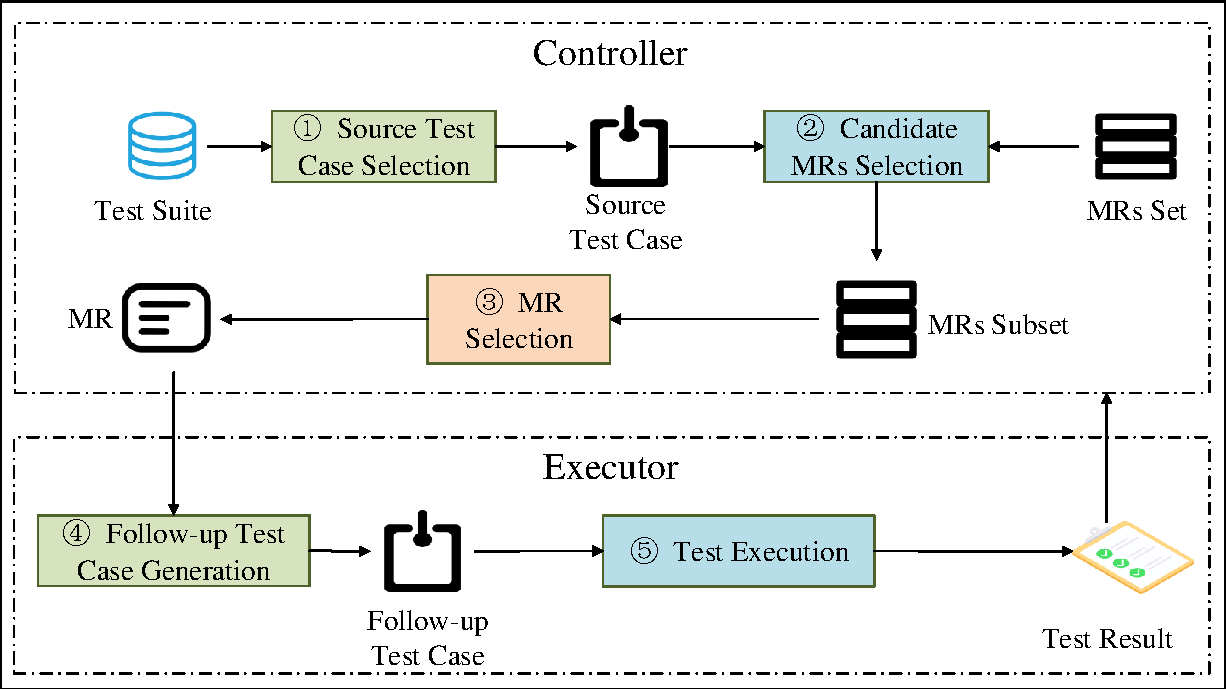
\includegraphics[width = 0.5\textwidth]{fig//generateframework}
  \caption{The Framework of AMT}
  \label{fig:framework}
\end{figure}

\begin{enumerate}[1]
  \item
  \emph{Source Test Case Selection}.

  \item
  \emph{candidate MRs Selection}.

  \item
  \emph{MR Selection}.

  \item
  \emph{Follow-up Test Case Generation}.

  \item
  \emph{Test Case Execution}.
  The relevant DRT component receives the generated test case, converts it into an input message, invokes the web service(s) through the SOAP protocol, and intercepts the test results (from the output message).
\end{enumerate}

\subsection{Updating Test Profile}
\label{sec:updatingTestProfile}
When the source test case $stc$ and follow-up test case $ftc$ related to an metamorphic relation $MR$ belong to the same partition $s_i$, DRT is suitable to adjust the test profile. However, during the test process, there are some scenarios where the $stc$ is not in the same partition as $ftc$. In such scenarios, DRT cannot be used to adjust the test profile. To solve this problem, we proposed metamorphic dynamic random testing (MDRT).

Suppose that source test case $stc$ and follow-up test case $ftc$ related to an metamorphic relation $MR$, belong to $s_i$ and $s_f$ ($f \in \{1, 2, \ldots, m\}, f \ne i$), respectively. If their results violate the $MR$, $\forall j = 1, 2, \ldots, m$ and $j \ne i, f$, we set

\begin{equation}
\label{eq:MDRThitJ}
p'_j =
\begin{cases}
p_j - \displaystyle\frac{2\epsilon}{m-2} & \text{if } p_j \geq \displaystyle\frac{2\epsilon}{m-2} \\
0 & \text{if } p_j < \displaystyle\frac{2\epsilon}{m-2}
\end{cases},
\end{equation}
where $\epsilon$ is a probability adjusting factor, and then

\begin{equation}
\label{eq:MDRThitI}
  p'_i = p_i + \displaystyle\frac{(1-\sum_{\substack{j = 1, j \ne i,m}}^m p_j^{'}) - p_i - p_f}{2},
\end{equation}

\begin{equation}
\label{eq:MDRThitF}
  p'_f = p_f + \displaystyle\frac{(1-\sum_{\substack{j = 1, j \ne i,m}}^m p_j^{'}) - p_i - p_f}{2}.
\end{equation}

Alternatively, if their results hold the $MR_h$, we set

\begin{equation}
\label{eq:MDRTmissI}
p'_i =
\begin{cases}
p_i - \epsilon & \text{if } p_i \geq \epsilon \\
0 & \text{if } p_i < \epsilon
\end{cases},
\end{equation}

\begin{equation}
\label{eq:MDRTmissF}
p'_f =
\begin{cases}
p_f - \epsilon & \text{if } p_f \geq \epsilon \\
0 & \text{if } p_f < \epsilon
\end{cases},
\end{equation}
and then for $\forall j = 1, 2, \ldots, m$ and $j \neq i, f$, we set

\begin{equation}
\label{eq:MDRTmissJ}
p'_j = p_j + \displaystyle\frac{(p_i - p_i^{'}) + (p_f - p_f^{'})}{m - 2}
\end{equation}

The detailed MDRT algorithm is given in Algorithm \ref{alg:mdrt}. In MDRT, the source test case is selected from a partition that has been randomly selected according to the test profile $\{\left \langle s_1, p_1 \right \rangle, \left \langle s_2, p_2 \right \rangle, \ldots, \left \langle s_m, p_m \right \rangle\}$, and an metamorphic relation is select according to some strategies (Lines 2 to 4 in Algorithm \ref{alg:drt}). During the testing, if the source and follow-up test cases are not in same partition, then the test profile is updated by changing the $p_i$: If a fault is detected, then Formulas \ref{eq:MDRThitJ}, \ref{eq:MDRThitI}, and \ref{eq:MDRThitF} are used to adjust the values of $p_i$ (Line 8), otherwise Formulas \ref{eq:MDRTmissI}, \ref{eq:MDRTmissF}, and \ref{eq:MDRTmissJ} are used (Line 10). The testing process is stopped as long as the termination condition is satisfied.

\begin{algorithm}
\caption{MDRT}
\label{alg:mdrt}
    \begin{algorithmic}[1]
    \renewcommand{\algorithmicrequire}{\textbf{Input:}}
    \renewcommand{\algorithmicendwhile}{\algorithmicend\_\algorithmicwhile}
    \renewcommand{\algorithmicendif}{\algorithmicend\_\algorithmicif}
    \REQUIRE $\epsilon, p_1, p_2, \ldots, p_m, MR_1, MR_2, \ldots, MR_n$
    \WHILE {termination condition is not satisfied}
    \STATE Select a partition $s_i$ according to the test profile $\{\left \langle s_1, p_1 \right \rangle, \left \langle s_2, p_2 \right \rangle, \ldots, \left \langle s_m, p_m
    \right \rangle\}$.
    \STATE Select a source test case $stc_i$ from $s_i$, and an metamorphic relation $MR_h$ ($h \in \{1, 2, \ldots, n\}$).
    \STATE Based on the $MR_h$, follow-up test case $ftc_i$ is generated from $stc_i$, belonging to partition $s_f$.
    \STATE Test the SUT using $stc_i$ and $ftc_i$.
    \IF {$i \ne f$}
    \IF {the results of $stc_i$ and $ftc_i$ violate the MR}
    \STATE Update $\{\left \langle s_1, p_1 \right \rangle, \left \langle s_2, p_2 \right \rangle, \ldots, \left \langle s_m, p_m \right \rangle\}$ according to Formulas
    \ref{eq:MDRThitJ}, \ref{eq:MDRThitI}, and \ref{eq:MDRThitF}.
    \ELSE
    \STATE Update $\{\left \langle s_1, p_1 \right \rangle, \left \langle s_2, p_2 \right \rangle, \ldots, \left \langle s_m, p_m \right \rangle\}$ according to Formulas
    \ref{eq:MDRTmissI}, \ref{eq:MDRTmissF}, and \ref{eq:MDRTmissJ}.
    \ENDIF
    \ENDIF
    \ENDWHILE
    \end{algorithmic}
\end{algorithm}

\subsection{Selecting MR Strategies}
\label{sec:selectingMR}

In AMT, once a source test case is selected, the corresponding candidate MRs are available. We first proposed a simple strategy based on random mechanism to select an MR from the set of candidate MRs, then we proposed an innovative strategy to select an MR that can make the execution of follow-up test case as different as possible from the source test case.



\subsubsection{Randomly MR-Selection Strategy (RMRS)}
\label{sec:rsmr}

RSMR randomly selects an from the set of candidate MRs, which is a straightforward method without considering extra information.

\subsubsection{Properties-Based strategy of MR selection (PBMR)}
\label{sec:pbmr}

The fault-detection efficiency of MT highly dependent on the specific MRs that are used, and selecting effective MRs is thus a critical step when applying MT. Chen et al. reported that good metamorphic relations are those that can make the execution of the source-test case as different as possible to its follow-up test case. Moreover, They defined the ``difference among execution" as any aspects of program runs (e.g., paths traversed).
Before presenting the properties-based strategy of MR selection (PBMR), we first introduce a new metric called category-partition-based metric (CP-distance) that measures the distance between the source test cases and corresponding follow-up test cases. CP-distance makes use of the concepts of categories and choices from the CPM method described in Section \ref{sec:cpm}. CP-distance have the capacity to reflect the difference among the source test cases and follow-up test cases, since the categories and choices are defined based on the software functionalities.

More formally, let us denote the set of categories by $A = \{A_1, A_2, \ldots, A_g\}$, where $g$ denotes the total number of categories. For each $A_i$, its choices are denotes by $P_i^{A_i} = \{p_1^{A_i},p_2^{A_i}, \ldots, p_h^{A_i}\}$, where $h$ denotes the number of choices for $A_i$. For input $x$, let us denote the corresponding non-empty subset by $A(x) = \{A_1^{x}, A_2^{x}, \ldots, A_q^{x}\}$, where $q$ refers to the number of categories associated with $x$. Since categories are distinct and their choices are disjoint, input $x$ in fact consists of values chosen from a non-empty subset of choices, denoted as $P(x) = \{p_1^{x}, p_2^{x}, \ldots, p_q^{x}\}$, where $p_i^x (i = 1, 2, \ldots, q)$ is the choice of the category $A_i^{x}$  for $x$.

For any two inputs $x$ and $y$, we define $DP(x,y)$ as the set that contains elements in either $P(x)$ or $P(y)$ but not both. That is,
$$DP(x,y) = (P(x) \cup P(y))\\ (P(x) \cap P(y)),$$ where ``n" is the set difference operator. Now, we define $$DA(x, y) = \{A_m|A_i if p_j^i \in DP(x, y)\}.$$ In other words, $DA(x, y)$ is the set of categories in which inputs $x$ and $y$ have different choices. Then, the distance measure between $x$ and $y$ is defined as $|DA(x, y)|$ (the size of $DA(x, y)$); that is, the number of categories that appear in either $x$ or $y$ but not both, or in which the choices in $x$ and $y$ differ.

obviously, a greater value of CP-distance representing more dissimilar execution. After selecting a source test case $stc_i$ and obtaining a set of candidate MRs $\mathcal{R} = \{r_1^{stc_i}, r_2^{stc_i}, \ldots, r_g^{stc_i}\}$ ($g$ is the number of MRs whose source test case could be $stc_i$), PBMR generate a set of candidate folow-up test cases $FC = \{ftc_{r_1^{stc_i}}, ftc_{r_2^{stc_i}}, \ldots, ftc_{r_g^{stc_i}}\}$ according to every MR belonged to $FC$. Then, the distance $CP_{i,h}$ ($h \in \{1,2, \ldots, g\}$) between $stc_i$ and each follow-up test case $ftc_{r_h^{stc_i}}$ is calculated. Finally, the MR $r_h^{stc_i}$ is selected as long as the following condition is hold:
$$CP_{i,h} = max\{CP_{i,1}, CP_{i,2}, \ldots, CP_{i,g}\}.$$

The details of PBMR is given in Algorithm \ref{alg:pbmr}.
\begin{algorithm}
\caption{PBMR}
\label{alg:pbmr}
    \begin{algorithmic}[1]
    \renewcommand{\algorithmicrequire}{\textbf{Input:}}
    \renewcommand{\algorithmicensure}{\textbf{Output:}}
    \renewcommand{\algorithmicendwhile}{\algorithmicend\_\algorithmicwhile}
    \renewcommand{\algorithmicendif}{\algorithmicend\_\algorithmicif}
    \REQUIRE $stc_i, \mathcal{R} = \{r_1^{stc_i}, r_2^{stc_i}, \ldots, r_g^{stc_i}\}, CParray = null$
    \ENSURE $CP_{max}$ ($max \in \{1, 2, \ldots, g\}$)
    \FOR {$h=1 \to h=g$}
    \STATE Generate the follow-up test case $ftc_h$ according to the $stc_i$ and $r_h^{stc_i}$
    \STATE Calculate the distance $CP_{i,h}$ between the $stc_i$ and $ftc_h$
    \STATE Add $CP_{i,h}$ to the list $CParray$
    \ENDFOR
    \STATE Calculate the maximal value $CP_{max}$ ($max \in \{1, 2, \ldots, g\}$) in the list $CParray$
    \end{algorithmic}
\end{algorithm}




\subsection{Partition Based AMT (P-AMT)}
\label{sec:P-AMT}

\subsubsection{A partition-centric P-AMT}
\begin{figure}[htb]
  \centering
  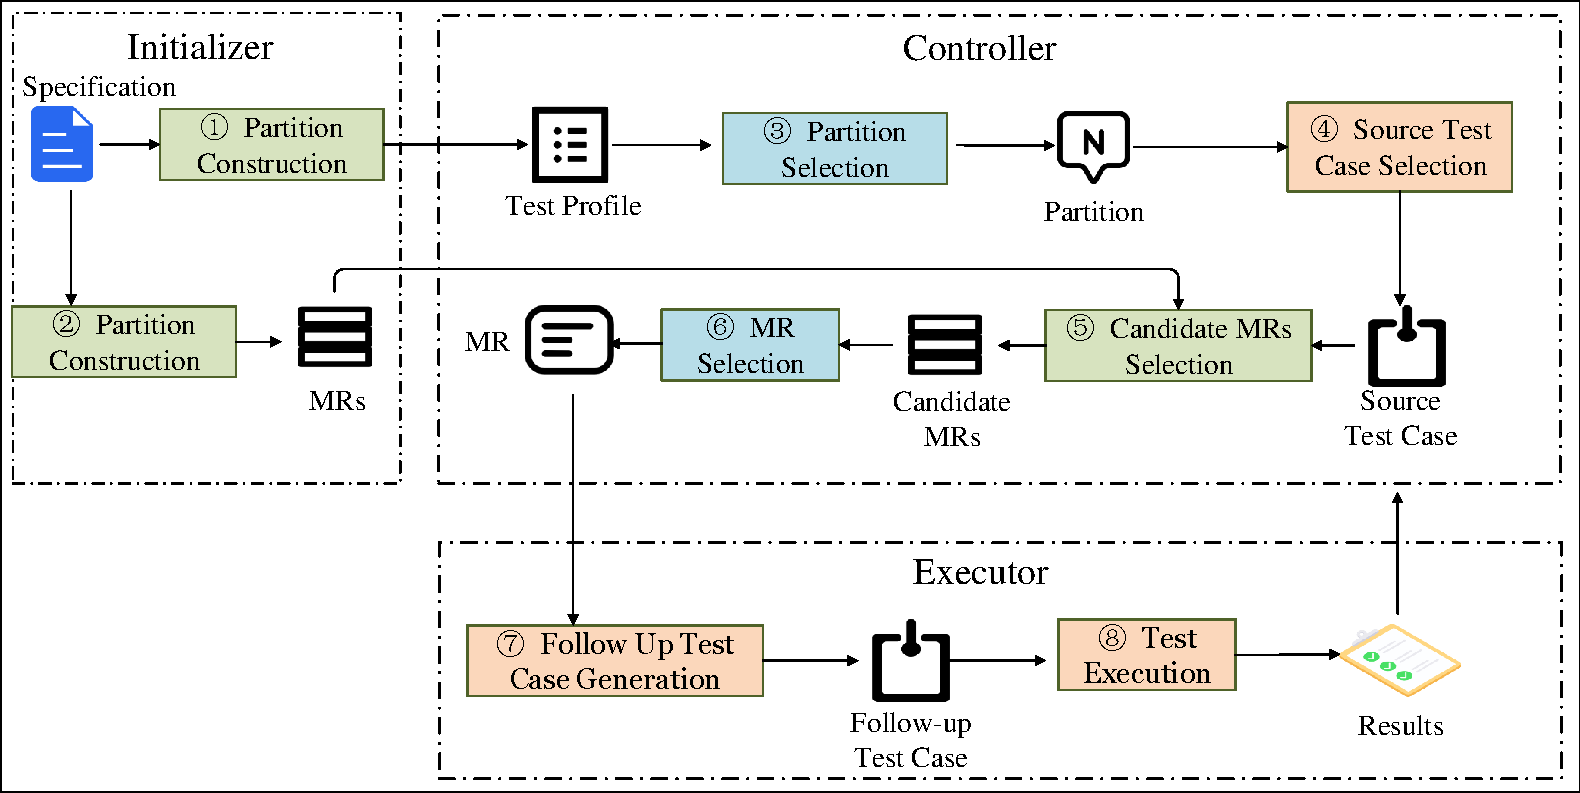
\includegraphics[width = 0.5\textwidth]{fig//pcenterpartitionframework}
  \caption{framework}
  \label{fig:The Framework of PP-AMT}
\end{figure}

\begin{algorithm}
\caption{PP-AMT}
\label{alg:pp-pfmt}
    \begin{algorithmic}[1]
    \renewcommand{\algorithmicrequire}{\textbf{Input:}}
    \renewcommand{\algorithmicendwhile}{\algorithmicend\_\algorithmicwhile}
    \renewcommand{\algorithmicendif}{\algorithmicend\_\algorithmicif}
    \REQUIRE $\epsilon, p_1, \ldots, p_m, MR_{s_1}, \ldots, MR_{s_m}, \mathcal{R}, counter$
    \STATE Initialize $counter = 1$.
    \WHILE {termination condition is not satisfied}
    \IF {$counter = 1$}
    \STATE Randomly select an $MR$ from $\mathcal{R}$, and $MR \in MR_{s_i}$.
    \STATE Increment counter by 1.
    \STATE Randomly select a source test case from the partition $s_i$, and generate the follow-up test case belonged to partition $s_f$ ($f \in {1,2,\ldots,m}$).
    \STATE Execute the source and follow-up test cases.
    \IF {the results of source and follow-up test cases violate $MR$}
    \IF {$i = f$}
    \STATE Update the test profile according to Formulas \ref{eq:DRThitJ} and \ref{eq:DRThitI}.
    \ELSE
    \STATE Update the test profile according to Formulas \ref{eq:MDRThitJ}, \ref{eq:MDRThitI}, and \ref{eq:MDRThitF}.
    \ENDIF
    \ELSE
    \IF {$i = f$}
    \STATE Update the test profile according to Formulas \ref{eq:DRTmissI} and \ref{eq:DRTmissJ}.
    \ELSE
    \STATE Update the test profile according to Formulas \ref{eq:MDRTmissI}, \ref{eq:MDRTmissF}, and \ref{eq:MDRTmissJ}
    \ENDIF
    \ENDIF
    \ELSE
    \STATE Select a partition $s_i$ according to the updated test profile, and then select an $MR^{'}$ from $MR_{s_i}$.
     \STATE Randomly select a source test case from the partition $s_i$, and generate the follow-up test case belonged to partition $s_f$ ($f \in {1,2,\ldots,m}$).
    \STATE Execute the source and follow-up test cases.
    \IF {the results of source and follow-up test cases violate $MR^{'}$}
    \IF {$i = f$}
    \STATE Update the test profile according to Formulas \ref{eq:DRThitJ} and \ref{eq:DRThitI}.
    \ELSE
    \STATE Update the test profile according to Formulas \ref{eq:MDRThitJ}, \ref{eq:MDRThitI}, and \ref{eq:MDRThitF}.
    \ENDIF
    \ELSE
    \IF {$i = f$}
    \STATE Update the test profile according to Formulas \ref{eq:DRTmissI} and \ref{eq:DRTmissJ}.
    \ELSE
    \STATE Update the test profile according to Formulas \ref{eq:MDRTmissI}, \ref{eq:MDRTmissF}, and \ref{eq:MDRTmissJ}
    \ENDIF
    \ENDIF
    \ENDIF
    \ENDWHILE
    \end{algorithmic}
\end{algorithm}





\subsubsection{A MRs-centric P-AMT (MP-AMT)}
\label{sec:mp-amt}

\begin{figure}[htb]
  \centering
  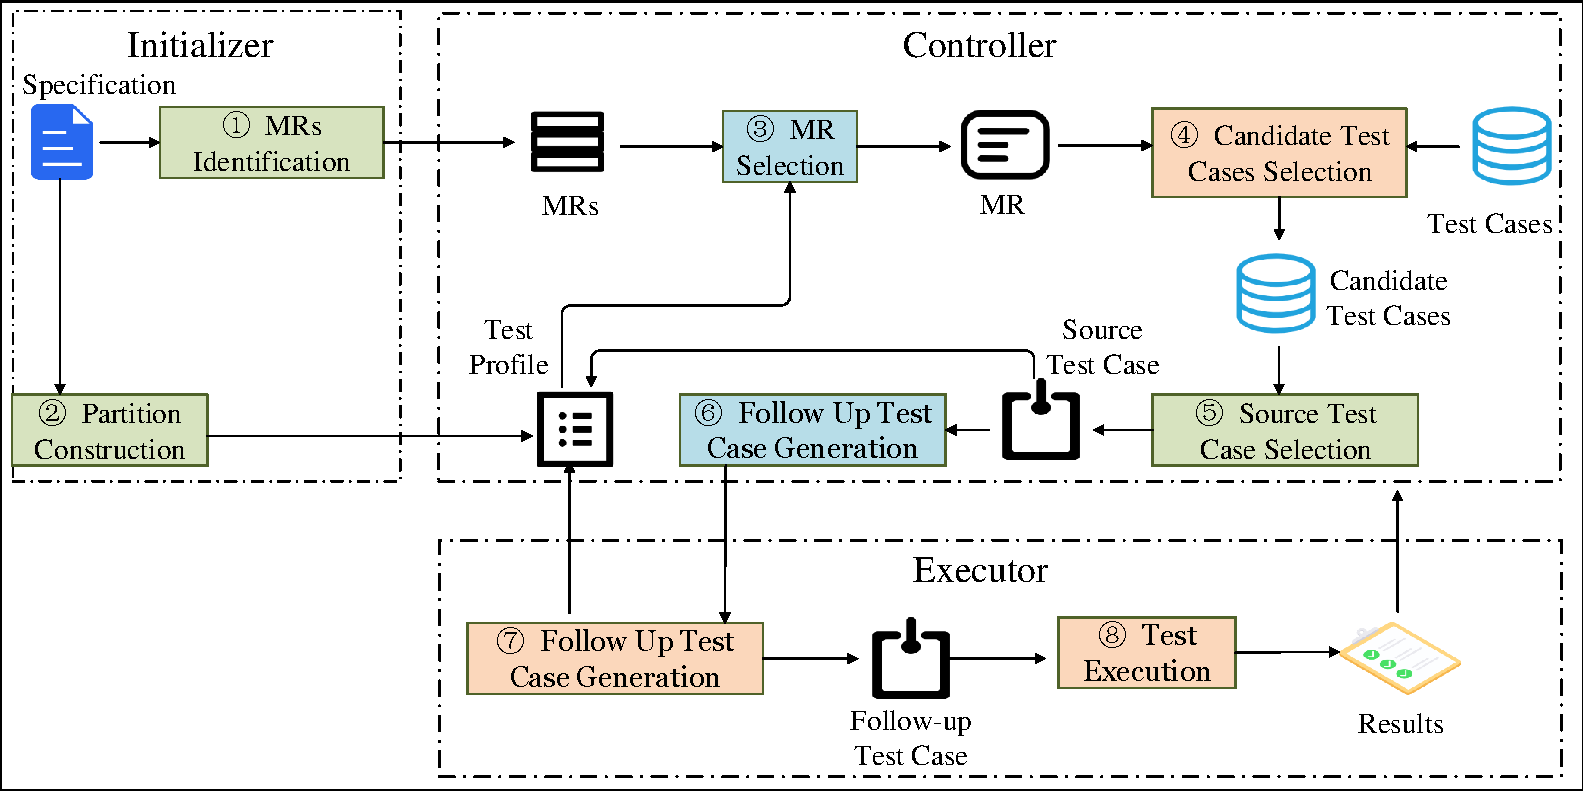
\includegraphics[width = 0.47\textwidth]{fig//mrscentricframework}
  \caption{The Framework of MP-AMT}
  \label{fig:framework}
\end{figure}

MRs-centric adaptive metamorphic testing (MP-AMT) adds a feedback mechanism to control the execution process of traditional MT. First, MP-AMT randomly selects an MR and a source test case belonging to a partition that is selected according to the test profile, generating the follow-up test case depend on the source test case, and then updates the test profile according to the result of test execution. Second, a partition is selected according to updated test profile, and an MR is randomly selected from the set of MRs whose source test case belong to selected partition.

Suppose that the input domain of SUT is divided into $m$ ($m > 2$) partitions ($s_1, s_2, \ldots, s_m$). A set $MR_{s_i}$ included metamorphic relations whose source test cases belong to the partition $s_i$, and $\mathcal{R} = \bigcup_{\substack{i = 1}}^mMR_{s_i}$ is a set that include all of metamorphic relations. The detailed MP-AMT algorithm is given in Algorithm \ref{alg:pm-pfmt}. In MP-AMT, the first metamorphic relation $MR$ is randomly selected from $\mathcal{R}$, and a source test case $stc$ is randomly selected from a partition $s_i$ related to the selected metamorphic relation, then the follow-up test case $ftc$ is generate based on $MR$ and $stc$, belonging to partition $s_f$ ($f \in \{1,2,\ldots, m\}$) (Lines 3 to 7 in Algorithm \ref{alg:pm-pfmt}). If the results of $stc$ and $ftc$ violate the $MR$, there are following two situation, denoted $\delta_1, \delta_2$, respectively (Lines 8 to 12):
\begin{enumerate}[ {Situation} 1 ($\delta_1$):]
  \item
  If $i = f$, then the test profile is updated according to Formulas \ref{eq:DRThitJ} and \ref{eq:DRThitI}.
  \item
  If $i \ne f$, then the test profile is updated according to Formulas \ref{eq:MDRThitJ}, \ref{eq:MDRThitI}, and \ref{eq:MDRThitF}.
\end{enumerate}

Alternatively, if their results satisfy the $MR$, there are following two situation, denoted $\delta_1^{'}, \delta_2^{'}$, respectively (Lines 14 to 18):
\begin{enumerate}[ {Situation} 1 ($\delta_1^{'}$):]
  \item
  If $i = f$, then the test profile is updated according to Formulas \ref{eq:DRTmissI} and \ref{eq:DRTmissJ}.

  \item
  If $i \ne f$, then the test profile is updated according to Formulas \ref{eq:MDRTmissI}, \ref{eq:MDRTmissF}, and \ref{eq:MDRTmissJ}.
\end{enumerate}

Next, MP-AMT randomly selects a partition according to updated test profile, then a source test case is randomly selected from the selected partition and an metamorphic relation is randomly selected from a $MR_{s_i}$ ($i \in \{1,2,\ldots,m\}$) whose source test cases belong to the selected partition. On the basis of $MR_{s_i}$, the follow-up test case is generated from the source test case (Lines 22 and 23). After the execution of the source and follow-up test cases, their results are verified against the $MR_{s_i}$, then the test profile is updated (Lines 24 to 35). This process is repeated until a termination condition is satisfied (Line 2).

We developed a tool called AMTester to the best of our knowledge. AMTester has features such as termination condition setting, partition setting, test execution, and test report generation.


\begin{algorithm}
\caption{MP-AMT}
\label{alg:pm-pfmt}
    \begin{algorithmic}[1]
    \renewcommand{\algorithmicrequire}{\textbf{Input:}}
    \renewcommand{\algorithmicendwhile}{\algorithmicend\_\algorithmicwhile}
    \renewcommand{\algorithmicendif}{\algorithmicend\_\algorithmicif}
    \REQUIRE $\epsilon, p_1, \ldots, p_m, MR_{s_1}, \ldots, MR_{s_m}, \mathcal{R}, counter$
    \STATE Initialize $counter = 1$.
    \WHILE {termination condition is not satisfied}
    \IF {$counter = 1$}
    \STATE Randomly select an $MR$ from $\mathcal{R}$, and $MR \in MR_{s_i}$.
    \STATE Increment counter by 1.
    \STATE Randomly select a source test case from the partition $s_i$, and generate the follow-up test case belonged to partition $s_f$ ($f \in {1,2,\ldots,m}$).
    \STATE Execute the source and follow-up test cases.
    \IF {the results of source and follow-up test cases violate $MR$}
    \IF {$i = f$}
    \STATE Update the test profile according to Formulas \ref{eq:DRThitJ} and \ref{eq:DRThitI}.
    \ELSE
    \STATE Update the test profile according to Formulas \ref{eq:MDRThitJ}, \ref{eq:MDRThitI}, and \ref{eq:MDRThitF}.
    \ENDIF
    \ELSE
    \IF {$i = f$}
    \STATE Update the test profile according to Formulas \ref{eq:DRTmissI} and \ref{eq:DRTmissJ}.
    \ELSE
    \STATE Update the test profile according to Formulas \ref{eq:MDRTmissI}, \ref{eq:MDRTmissF}, and \ref{eq:MDRTmissJ}
    \ENDIF
    \ENDIF
    \ELSE
    \STATE Select a partition $s_i$ according to the updated test profile, and then select an $MR^{'}$ from $MR_{s_i}$.
     \STATE Randomly select a source test case from the partition $s_i$, and generate the follow-up test case belonged to partition $s_f$ ($f \in {1,2,\ldots,m}$).
    \STATE Execute the source and follow-up test cases.
    \IF {the results of source and follow-up test cases violate $MR^{'}$}
    \IF {$i = f$}
    \STATE Update the test profile according to Formulas \ref{eq:DRThitJ} and \ref{eq:DRThitI}.
    \ELSE
    \STATE Update the test profile according to Formulas \ref{eq:MDRThitJ}, \ref{eq:MDRThitI}, and \ref{eq:MDRThitF}.
    \ENDIF
    \ELSE
    \IF {$i = f$}
    \STATE Update the test profile according to Formulas \ref{eq:DRTmissI} and \ref{eq:DRTmissJ}.
    \ELSE
    \STATE Update the test profile according to Formulas \ref{eq:MDRTmissI}, \ref{eq:MDRTmissF}, and \ref{eq:MDRTmissJ}
    \ENDIF
    \ENDIF
    \ENDIF
    \ENDWHILE
    \end{algorithmic}
\end{algorithm}

\subsection{Random Based AMT (R-AMT)}
\label{sec:ramt}

Random Testing (RT) tests software by randomly generating inputs, which is a standard black-box software testing technique. The IEEE Guide to the Software Engineering Body of Knowledge (SWEBOK) \cite{bourque2014guide} lists RT as one of four common input-domain based testing techniques, along with equivalence partitioning, pairwise testing, and boundary value analysis. Arcuri et al. \cite{arcuri2012random} observe that RT is one of the most used automated testing techniques in practice. Therefore, we particularly develop one algorithm, random based AMT (R-AMT), to implement the proposed AMT. The framework of R-AMT is illustrated in Figure \ref{fig:rtframework}.
\begin{figure}[htb]
  \centering
  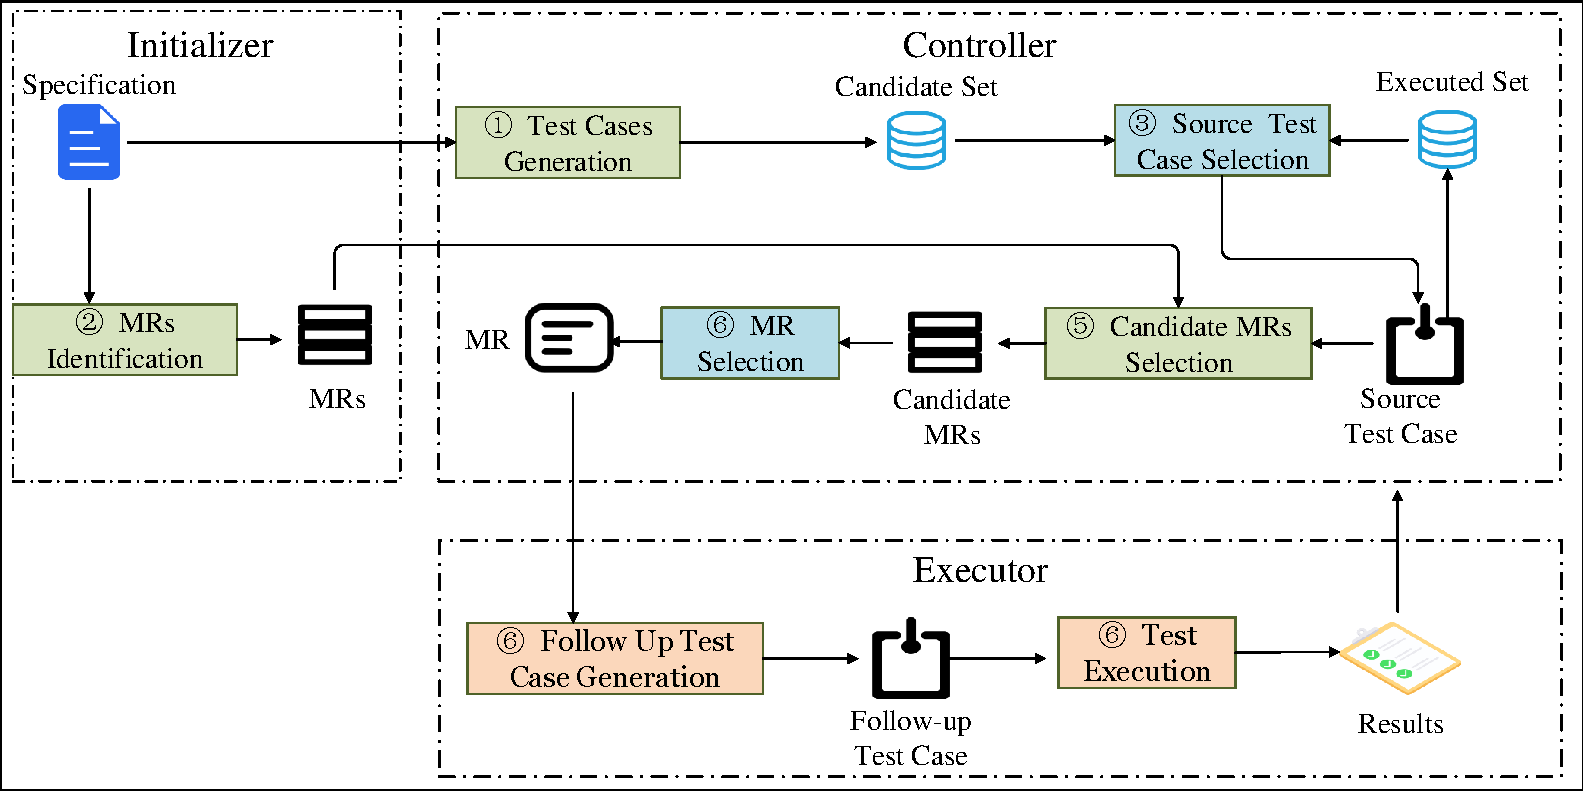
\includegraphics[width = 0.47\textwidth]{fig//rtframework}
  \caption{The Framework of R-AMT}
  \label{fig:rtframework}
\end{figure}

In R-AMT, we make use the ARTsum algorithm to generate source test cases. Accordingly, a set of candidate MRs $\mathcal{CR}$ can be obtained according to the selected source test case. Then, an MR is selected by using the proposed RMRS or PBMR strategy. The details of R-AMT is given in Algorithm \ref{alg:R-pfmt}


\begin{algorithm}
\caption{R-AMT}
\label{alg:R-pfmt}
    \begin{algorithmic}[1]
    \renewcommand{\algorithmicrequire}{\textbf{Input:}}
    \renewcommand{\algorithmicendwhile}{\algorithmicend\_\algorithmicwhile}
    \renewcommand{\algorithmicendif}{\algorithmicend\_\algorithmicif}
    \REQUIRE $\mathcal{R} $
    \WHILE {termination condition is not satisfied}
    \STATE Generate a source test case $stc_i$ using the Algorithm \ref{alg:artsum}.
    \STATE Select the MR from $\mathcal{R}$, whose source test case can be $stc_i$ and add the selected MR to $\mathcal{CR}$
    \STATE Select an MR $MR_s$ form $\mathcal{CR}$ using the proposed strategy RMRS or PBMR.
    \STATE Generate the follow-up test case $ftc_i$ according to $stc_i$ and $MR_s$.
    \STATE Test the software using the $stc_i$ and $ftc_i$.
    \STATE Verify the outputs of $stc_i$ and $ftc_i$ against the $MR_s$.
    \ENDWHILE
    \end{algorithmic}
\end{algorithm}


\section{Empirical Study}
\label{sec:empiricalStudy}

We conducted a series of empirical studies to evaluate the performance of DRT.

\subsection{Research Questions}
\label{sec:rqs}
In our experiments, we focused on addressing the following three research questions:
\begin{description}
  \item [\textbf{RQ1}] \textbf{How efficient is AMT at detecting faults?}

  Fault-detection efficiency is a key criterion for evaluating the performance of a testing technique. In our study, we chose three real-life programs, and applied mutation analysis to evaluate the fault-detecting efficiency.

  \item [\textbf{RQ2}] \textbf{What is the actual test case selection overhead when using the AMT technique?}

  We evaluate the test case selection overhead of M-AMT and compare with traditional MT in detecting software faults.
\end{description}

\subsection{Object Programs}
\label{sec:programs}

In order to evaluate the fault-detection effectiveness of proposed methods in different scales, different implementation languages, and different fields, we chose to study four sets of object programs: three laboratorial programs that were developed according to corresponding specifications, seven programs from the Software-artifact Infrastructure Repository (SIR) \cite{do2005supporting}, the regular expression processor component of the larger utility program \texttt{GUN grep}, and a Java library developed by Alibaba, which can be used to convert Java Objects into their JSON representation, and convert a JSON string to an equivalent Java object. The details of twelve programs are summarized in Table \ref{table:objects}.


\begin{table*}[hbt]
  \caption{Twelve Programs as Experimental Objects}
  \label{table:objects}
  \centering
  \begin{tabular}{llllllll} \toprule
  \multirow{2}{*}{Source}&\multirow{2}{*}{Programs}&\multirow{2}{*}{Language}&\multirow{2}{*}{LOC}&\multirow{2}{*}{All Faults}
  &\multirow{2}{*}{Used Faults} &Number of  &Number of  \\
  & & & &          &            &MRs        &Partitions\\ \midrule
                                &\texttt{CUBS}        &Java      &107     &187        &4           &184        &8 \\ 
  \multirow{2}{*}{Laboratory}   &\texttt{ACMS}        &Java      &128     &210        &9           &142        &4 \\ 
								&\texttt{ERS}         &Java      &117     &180        &4           &1130       &12 \\ 
								&\texttt{MOS}         &Java      &135     &215        &1           &3512       &9  \\ \midrule
  \multirow{7}{*}{SIR}          &\texttt{printtokens} &C         &483     &7          &7           &3          &-- \\ 
    							&\texttt{printtokens2}&C         &402     &10         &10          &3          &-- \\ 
         						&\texttt{replace}     &C         &516     &31         &31          &3          &-- \\ 
        						&\texttt{schedule}    &C         &299     &9          &9           &3          &-- \\ 
       							&\texttt{schedule2}   &C         &297     &9          &9           &3          &-- \\ 
            					&\texttt{tcas}        &C         &138     &41         &41          &3          &-- \\ 
         						&\texttt{totinfo}     &C         &346     &23         &23          &3          &552 \& 3380 \\\midrule
  GUN                           &\texttt{grep}        &C         &10,068  &20         &20          &12         &-- \\ \midrule
  Alibaba                       &\texttt{FastJson}    &Java      &204125  &6          &6           &--         &-- \\ \bottomrule
  \end{tabular}
\end{table*}



There four sets of programs present complementary strengths and weaknesses as experiment objects. The Laboratorial programs implement simple functions and their interfaces are easy to understand. The test engineers can easily generate source test cases, and identify MRs for testing laboratorial programs. However, these programs are small and there are a limited number of faulty versions available for each programs. The SIR repositories provides object programs, including a number of pre-existing versions with seeded faults, as well as a test suite in which test cases were randomly generated. It is a challenge task to partition the input domain of those programs. The \texttt{grep} program is a much larger system for which mutation faults could be generated. The \texttt{FastJson} is also a much larger system, and the faults of that are obtained on GitHub.
We provide further details on each of those sets of object programs next.

\subsubsection{Laboratorial Programs}
\label{sec:labPrograms}

Based on three real-lift specifications, We developed three systems, respectively. \texttt{China Unicom Billing System (CUBS)} provides an interface through which customers can know how much they need to pay according to plans, month charge, calls, and data usage. The details of two cell-phone plans are summarized in Tables \ref{table:chinaA} and \ref{table:chinaB}. \texttt{Aviation Consignment Management System (ACMS)} aims to help airline companies check the allowance (weight) of free baggage, and the cost of additional baggage. Based on the destination, flights are categorized as either domestic or international. For international flights, the baggage allowance is greater if the passenger is a student (30kg), otherwise it is 20kg. Each aircraft offers three cabins classes from  which to choose (economy, business, and first), with passengers in different classes having different allowances. The detailed price rules are summarized in Table~\ref{table:acms}, where $price_0$ means economy class fare.
\texttt{Expense Reimbursement System (ERS)} assists the sales Supervisor of a company with handling the following tasks: \rmnum{1}) Calculating the cost of the employee who use the cars based on their titles and the number of miles actually traveled; \rmnum{2}) accepting the requests of reimbursement that include airfare, hotel accommodation, food and cell-phone expenses of the employee.

\begin{table}[!htp]
  \centering
  \caption{Plan A}
  \label{table:chinaA}
  \resizebox{0.46\textwidth}{!}{
  \begin{tabular}{|c|c|c|c|c|c|} \hline
  \multicolumn{2}{|c|}{\multirow{2}{*}{Plan details}}  &\multicolumn{4}{|c|}{Month charge~(CNY)} \\ \cline{3-6}
  \multicolumn{2}{|c|}{}                                     &\!$option_1$\!  &\!$option_2$\!  &\!$option_3$\! &\!$option_4$\! \\ \hline
   \multirow{2}{*}{\rotatebox{90}{Basic}} &Free calls~(min)  &50  &96  &286 &3000   \\ \cline{2-6}
                                          &Free data~(MB)    &150 &240 &900 &3000\\ \hline
   \multirow{2}{*}{\rotatebox{90}{Extra}} &Dialing calls~(CNY/min)  &0.25 &0.15  &0.15 &0.15 \\ \cline{2-6}
                                          &Data~(CNY/KB)  &\multicolumn{4}{c|}{0.0003} \\ \hline
  \end{tabular}}
\end{table}

\begin{table}[!htp]
  \caption{Plan B}
  \label{table:chinaB}
  \centering
  \resizebox{0.46\textwidth}{!}{
  \begin{tabular}{|c|c|c|c|c|c|} \hline
  \multicolumn{2}{|c|}{\multirow{2}{*}{Plan details}}  &\multicolumn{4}{|c|}{Month charge~(CNY)} \\ \cline{3-6}
  \multicolumn{2}{|c|}{}                                     &\!$option_1$\!  &\!$option_2$\!  &\!$option_3$\! &\!$option_4$\! \\ \hline
   \multirow{2}{*}{\rotatebox{90}{Basic}} &Free calls~(min)  &120  &450  &680 &1180   \\ \cline{2-6}
                                          &Free data~(MB)    &40 &80 &100 &150\\ \hline
   \multirow{2}{*}{\rotatebox{90}{Extra}} &Dialing calls~(CNY/min)  &0.25 &0.15  &0.15 &0.15 \\ \cline{2-6}
                                          &Data~(CNY/KB)  &\multicolumn{4}{c|}{0.0003} \\ \hline
  \end{tabular}}
\end{table}


\begin{table*}[!htp]
  \caption{ACMS Baggage Allowance and Pricing Rules}
  \label{table:acms}
  \centering
  \begin{tabular}{|c|c|c|c|c|c|c|} \hline
  \multirow{2}{*}{}     &\multicolumn{3}{c|}{Domestic flights}              &\multicolumn{3}{c|}{International flights} \\ \cline{2-7}
                                    &First class  &Business class   &Economy class   &First class  &Business class   &Economy class \\ \hline
  Carry~on (kg)                     &5       &5        &5        &7        &7        &7  \\ \hline
  Free checked-in (kg)              &40      &30       &20       &40       &30       &20/30 \\ \hline
  Additional baggage pricing~(kg)   &\multicolumn{3}{c|}{$price_0 * 1.5\%$}   &\multicolumn{3}{c|}{$price_0 * 1.5\%$}  \\ \hline
  \end{tabular}
\end{table*}

\subsubsection{SIR Programs}
\label{sec:SIRPrograms}

The seven object programs selected from the SIR [24] repository were \texttt{printtokens}, \texttt{printtokens2}, \texttt{replace}, \texttt{schedule}, \texttt{schedule2}, \texttt{tcas}, and \texttt{totinfo}. These programs were originally compiled by Hutchins et al. \cite{hutchins1994experiments} at Siemens Corporate Research. We used these programs for several reasons:
\begin{enumerate}[1]
  \item
  Faulty versions of the programs are available.

  \item
  The programs are of manageable size and complexity for an initial study.

  \item
  All programs and related materials are available from the SIR, and the MRs of each program are defined in  \cite{xie2013metamorphic}.

\end{enumerate}

The \texttt{printtokens} and \texttt{printtokens2} are independent implementations of the same specification. They each implement a lexical analyzer. Their input files are split into lexical tokens according to a tokenizing scheme, and their output is the separated tokens. The \texttt{replace} program is a command-line utility that takes a search string, a replacement string, and an input file. The search string is a regular expression. The replacement string is text, with some metacharacters to enable certain features. The \texttt{replace} program searches for occurrences of the search string in the input file, and produces an output file where each occurrence of the search string is replaced with the replacement string. The \texttt{schedule} and \texttt{schedule2} programs are also independent implementations of the same specification. They each implement a priority scheduler that takes three non-negative integers and an input file. The integers indicate the number of initial processes at the three available scheduling priorities. The \texttt{schedule} and \texttt{schedule2} programs then take as input a command file that specifies certain actions to be taken. The \texttt{tcas} program is a small part of a much larger aeronautical collision avoidance system. It performs simple analysis on data provided by other parts of the system and returns an integer indicating what action, if any, the pilot should take to avoid collision.

\subsubsection{GUN grep}
\label{sec:grep}

The used version of the \texttt{grep} programs is 2.5.1a \cite{grep}. This program searches one or more input files for lines containing a match to a specified pattern. By default, grep prints the matching lines. We chose \texttt{grep} for our study for several reasons:
\begin{enumerate}[1]
  \item
  \texttt{grep} program is wide used in Unix system, providing a opportunity to demonstrate the real world relevance of our techniques.
  \item
  \texttt{grep} program, and its input format, are of greater complexity than the the programs in the other test sets, but still manageable as a target for automated test case generation.
\end{enumerate}

The inputs of the \texttt{grep} were categorize into three components: options, which consist of a list of commands to modify the searching process, pattern, which is the regular expression to be searched for, and files, which refers to the input files to be searched.

The scope of functionality of this program is larger, which leads to construct test infrastructure to test all of functionality would have been impractical. Therefore, we restricted our focus to the regular expression analyzer of the \texttt{grep}.

\subsubsection{Real-World Popular Programs}
\label{sec:realPragrams}

\texttt{FastJson} is a Java library that can be used to convert Java Objects into their JSON representation. It can also be used to convert a JSON string to an equivalent Java object. We chose \texttt{FastJson} for our study for several reason:

\begin{enumerate}[1]
  \item
  \texttt{FastJson} is wide used in real-word projects, providing a opportunity to demonstrate the real world relevance of our techniques.
  \item
  \texttt{FastJson} is more complex than other programs, and it is a open source project, that is, we can obtain its faults freely and conveniently.
  \item
  The chosen version of \texttt{FastJson} is 1.2.48, which was reported that had many faults that can support our research.
\end{enumerate}



\subsection{Variables}

\subsubsection{Independent Variables}
\label{sec:independentvariables}

The independent variable in our experiment is the different strategies that improve the fault-detection efficiency. As choices for this variable, we include, of course, proposed PP-AMT, MP-AMT, and R-AMT. As baseline techniques for use in comparison, we selected two additional techniques, traditional MT and MT-ARTsum.

\begin{table}[htb]
  \caption{The Details of Independent Variables}
  \centering
  \label{table:independent}
  \begin{tabular}{llll} \toprule
  \multicolumn{2}{l}{\multirow{3}{*}{Techniques}}                          &The strategy of         &The strategy of \\
  \multicolumn{2}{l}{}                                                     &selecting Source        &selecting MRs   \\
  \multicolumn{2}{l}{}                                                     &Test Case               &             \\ \midrule
  \multicolumn{1}{l}{}                                 &PP-AMT             &MAPT                    &Random        \\ 
  \multicolumn{1}{l}{\multirow{1}{*}{Proposed}}        &PP-AMT*            &MAPT                    &PBMR          \\ 
  \multicolumn{1}{l}{\multirow{1}{*}{Techniques}}      &MP-AMT             &RAPT                    &Random        \\ 
  \multicolumn{1}{l}{}                                 &MP-AMT*            &RAPT                    &PBMR          \\ \midrule
  \multicolumn{1}{l}{}                                 &MT                 &Random                  &Random        \\ 
  \multicolumn{1}{l}{Baselines}                        &MT-ARTsum          &ARTsum                  &Random         \\ 
  \multicolumn{1}{l}}                                  &MT-DRT             &DRT                     &Random         \\
  \bottomrule
  \end{tabular}
\end{table}

Table \ref{table:independent} summarizes the details information of selecting source test cases and MRs of different techniques. Traditional MT is a natural baseline choice, because all proposed techniques is designed as an enhancement to MT, and assessing whether proposed techniques including PP-AMT, MP-AMT, and R-AMT is more cost-effective than MT is important.

There exist some techniques, such as quasi-random testing (QRT) \cite{ciupa2008artoo}, RBCVT-Fast \cite{shahbazi2013centroidal}, ARTmif \cite{chan2006forgetting}, and ARTsum \cite{barus2016cost} that can achieve a computation overhead as low as $O(n)$. However, QRT and RBCVT-Fast can be only to test software with an exclusively numeric input domain, and therefore could not be compared to proposed techniques. Moreover, Barus et al. \cite{barus2016cost} has been empirically shown that ARTsum had a much lower selection overhead than ARTmif, and its overhead was close to that of RT. Thus, we used ARTsum to select the source test cases of MT as one of baseline techniques.


\subsubsection{Dependent Variables}
\label{sec:dependentvariables}

The choice of a metric to use in comparing the effectiveness of testing techniques is non-trivial.

The dependent variable for RQ1 is the metric for evaluating the fault-detection effectiveness.
Several effectiveness metrics exist, including:
the P-measure~\cite{duran1984evaluation} (the probability of at least one fault being detected by a test suite);
the E-measure~\cite{chen1997optimal} (the expected number of faults detected by a test suite);
the F-measure~\cite{sun2018adaptive} (the expected number of test case executions required to detect the first fault); and
the T-measure~\cite{zhang2014history} (the expected number of test cases required to detect all faults).
Since the F- and P-measures have been widely used for evaluating the fault-detection efficiency and effectiveness of MT, ART, and DRT-related testing techniques~\cite{sun2018adaptive, barus2016cost, barus2016impact}, they are also adopted in this study. We use $F$ and $P$ to represent the F-measure and the P-measure of a testing technique.

We define $F$-$count$ as the number of test cases needed to detect a failure in a specific test run.
The F-measure is the expected $F$-$count$ for a testing method:

\begin{equation}
  \label{eq:fmeasure}
  F = \overline{F-count}.
\end{equation}
The F-measure is particularly appropriate for measuring the failure-detection effectiveness of adaptive testing methods, such as ART and DRT, in which the generation of new test cases depends on the previously executed test cases or the execution results of executed test case.

The $P$ can characterize the testing process. Suppose that a particular method is used to generate a test suite with $n$ test cases $\{t_1, t_2, \ldots, t_n\}$,  the $P$ is defined as the probability of at least one failure being detected by the test suite:

\begin{equation}
  \label{eq:pmeasure}
  P(n) = Prob(\exists t_i ~\text{that reveals a failure}).
\end{equation}
where $i = 1,2, \ldots, n$. A larger P reflects better failure-detection effectiveness.

The rate of occurrence of failures (ROCOF) that is the probability that a failure (not necessarily the first) occurs in a given interval of executions, which is relevant for operating systems where the system has to process a large number of similar requests that are relatively frequent.
ROCOF reflects the rate of occurrence of failure or anomalies in the system \cite{lyu1996handbook}.

Holm-Bonferroni method \cite{holm1979simple} to determine which pair of testing techniques have significant difference in terms of $F$. Across the whole study, for each pair of testing techniques, denoted by technique a and technique b, the null hypothesis ($H_0$) was that a and b had similar performance in terms of one metric; whereas the alternative hypothesis ($H_1$) was that a and b had significantly different performance in terms of $F$. All the null hypotheses were ordered by their corresponding p-values, from lowest to largest; in other words, for null hypotheses $H_0^1, H_0^2, \ldots, H_0^{h-1}$, we had $p_1 \leq p_2 \leq ...$ For the given confidence level $\alpha = 0.05$, we found the minimal index $h$ such that $p_h > \frac{\alpha}{N + 1 - h}$ (where N is the total number of null hypotheses). Then, we rejected $H_0^1, H_0^2, \ldots, H_0^{h-1}$, that is, we regarded the pair of techniques involved in each of these hypotheses to have statistically significant difference in terms of a certain metric.
On the other hand, we considered the pair of techniques involved in each of $H_0^h, H_0^{h + 1}, ...$ not to have significant difference with respect to one metric, as these hypotheses were accepted.


An obvious metric for RQ2 is the time required to detect faults. Corresponding to the T-measure, in this study we used $F$-$time$ denote the time required (i.e. test cases generation, test cases selection, and test cases execution) to detect the first fault. Obviously, a smaller values of $F$-$time$ indicate a better performance.



\subsection{Experimental Settings}

\subsubsection{Partitioning}
\label{sec:partition}

The proposed techniques PP-AMT and MP-AMT both based on the partition testing that is a mainstream family of software testing techniques, which can be realized in different ways, such as Intuitive Similarity, Equivalent Paths, Risk-Based, and Specified As Equivalent (two test values are equivalent if the specification says that the program handles them in the same way) \cite{kaner2010introduction}. In this study, we made use of the CPM to conduct the partitioning. Our previous work \cite{sun2018adaptive} found that there is not a strong correlation between the granularity level in partitioning and the performance of APT. Therefore, we Select two categories that have fewer choices annotated with [single] or [error], and partition the input domain according to the combinations of their choices.

We use an explanatory example to illustrate the method of partitioning. According to the description of Section \ref{sec:labPrograms},  we identify categories and associated choices of \texttt{ACMS}, as shown in Table \ref{table:categoryAndchoice}. With these categories/choices and constraints among choices, we further derive a set of complete test frames and each of them corresponds to a partition. Note that the number of partitions may vary with the granularity level. To ease the illustration, we derive partitions without considering the baggage weight category. Table \ref{table:partitionrule} shows the resulting partitions for BB, where $weight_*$ indicates no classification on the baggage weight.
\begin{table}
  \caption{Categories and choices of ACMS}
  \label{table:categoryAndchoice}
  \centering
  \begin{tabular}{ll}
  \toprule
  Category                    & Associated choices \\
  \midrule
   aircraft cabin             & \emph{Economy}, \emph{Business}, \emph{First Class} \\
   flight region              & \emph{International}, \emph{Domestic} \\
   baggage weight             & \emph{Above Limit}, \emph{Below Limit} \\
  \bottomrule
  \end{tabular}
\end{table}

\begin{table}
  \caption{Partitions of ACMS}
  \label{table:partitionrule}
  \centering
  \begin{tabular}{|l|l|} \hline
  Partition       & Complete Test Frame \\ \hline
  $c_1$  & \{$International$, $Economy$, $weight_*$ \} \\ \hline
  $c_2$  & \{$International$, $Business$, $weight_*$\} \\ \hline
  $c_3$  & \{$International$, $First Class$, $weight_*$\} \\ \hline
  $c_4$  & \{$Domestic$, $Economy$, $weight_*$ \} \\ \hline
  $c_5$  & \{$Domestic$, $Business$, $weight_*$\} \\ \hline
  $c_6$  & \{$Domestic$, $First Class$, $weight_*$\} \\ \hline
  \end{tabular}
\end{table}

\subsubsection{Initial Test Profile}
\label{sec:testprofile}

The proposed techniques PP-AMT and MP-AMT make use of feedback information to adjust the test profile. Then the updated test profile guide those techniques to select next source test case or MR. Before executing the test, a concrete test profile should be initialized. In our previous work \cite{sun2018adaptive}, we have compared the equal and proportional initial test profile in terms of associated performance metrics (F-measure, F2-measure \cite{sun2018adaptive}, and T-measure). The comparison results that there was no significant difference between these two types of initial test profiles. And as a result, we used a uniform probability distribution as the initial testing profile in this study.

\subsubsection{Constants}
\label{sec:constants}

In PP-AMT and MP-AMT, there is a parameter $\epsilon$ that is a probability adjusting factor. We followed studies \cite{Lv2011, Yang2014, li2015approach} to set $\epsilon = 0.05$.

In R-AMT, ARTsum is employed to generate source test cases, which has a parameter $k$ --- the size of the candidate set. Previous work \cite{chen2004adaptive} has shown that at least for numeric programs --- that failure detection effectiveness improves as $k$ increase up to about 10, and then does not improve much further. In addition, Barus \cite{barus2016cost} applied ARTsum to non-numeric programs where the value of $k$ was set 10. Therefore, our experiments were all conducted with $k$ set to 10.

\subsection{Generation of Categories and Choices for Object Programs}
\label{sec:generatecategories}

The categories and choices used for the laboratorial programs and Real-World Popular Programs considered in this study were designed by the authors. On the other hand, the categories and choices used for the SIR Programs and GUN Program were designed by Barus \cite{barus2016cost}. In large part, the selection of appropriate categories and choices is at a tester��s discretion; we chose what we regarded as simple approaches for emulating that process. Precise details on the categories and choices used in our study are provided as following.

\subsubsection{The categories and choices of Laboratorial Programs}
\label{sec:categoriesoflp}

\begin{table}[htb]
  \caption{Definition of Categories and Choices for \texttt{CUBS}}
  \label{table:categoriesofcubs}
  \centering
  \begin{tabular}{|c|c|c|} \hline
  \#               &Category                                                  &Choice   \\ \hline
  1                &\multicolumn{1}{c|}{\multirow{2}{*}{plan}}              &A        \\ \cline{3-3}
                   &\multicolumn{1}{c|}{}                                      &B         \\ \hline
  2                &\multicolumn{1}{c|}{\multirow{6}{*}{options}}              &46CNY     \\ \cline{3-3}
                   &\multicolumn{1}{c|}{}                                      &96CNY     \\ \cline{3-3}
                   &\multicolumn{1}{c|}{}                                      &286CNY     \\ \cline{3-3}
                   &\multicolumn{1}{c|}{}                                      &886CNY     \\ \cline{3-3}
                   &\multicolumn{1}{c|}{}                                      &126CNY     \\ \cline{3-3}
                   &\multicolumn{1}{c|}{}                                      &186CNY     \\ \hline
  3                &\multicolumn{1}{c|}{\multirow{2}{*}{calls}}                & calls $<$ free calls  \\ \cline{3-3}
                   &\multicolumn{1}{c|}{}                                      & calls $\geq$ free calls  \\ \hline
  4                &\multicolumn{1}{c|}{\multirow{2}{*}{data}}                 & data  $<$ free data  \\ \cline{3-3}
                   &\multicolumn{1}{c|}{}                                      & data $\geq$ free data  \\ \hline
  \end{tabular}
\end{table}

\begin{table}[htb]
  \caption{Definition of Categories and Choices for \texttt{ACMS}}
  \label{table:categoriesofacms}
  \centering
  \begin{tabular}{|c|c|c|} \hline
  \#               &Category                                                   &Choice      \\ \hline
  1                &\multicolumn{1}{c|}{\multirow{4}{*}{class}}                &first calss        \\ \cline{3-3}
                   &\multicolumn{1}{c|}{}                                      &Business class     \\ \cline{3-3}
                   &\multicolumn{1}{c|}{}                                      &Economy class       \\ \cline{3-3}
                   &\multicolumn{1}{c|}{}                                      &infant               \\ \cline{3-3}
  2                &\multicolumn{1}{c|}{\multirow{2}{*}{region}}               &Domestic flights     \\ \cline{3-3}
                   &\multicolumn{1}{c|}{}                                      &International flights    \\ \hline
  3                &\multicolumn{1}{c|}{\multirow{2}{*}{isStudent}}            &True                    \\ \cline{3-3}
                   &\multicolumn{1}{c|}{}                                      &False                   \\ \hline
  4                &\multicolumn{1}{c|}{\multirow{2}{*}{luggage}}              &luggage $<$ Free checked-in    \\ \cline{3-3}
                   &\multicolumn{1}{c|}{}                                      &luggage $\leq$ Free checked-in  \\ \hline
  5                &\multicolumn{1}{c|}{\multirow{2}{*}{fee}}                  &fee $=$ 0                      \\ \cline{3-3}
                   &\multicolumn{1}{c|}{}                                      &fee $\leq$ 0                   \\ \hline
  \end{tabular}
\end{table}


\begin{table}[htb]
  \caption{Definition of Categories and Choices for \texttt{ERS}}
  \label{table:categoriesofers}
  \centering
  \begin{tabular}{|c|c|c|} \hline
  \#               &Category                                                   &Choice      \\ \hline
  1                &\multicolumn{1}{c|}{\multirow{4}{*}{title}}                &senior sales manager        \\ \cline{3-3}
                   &\multicolumn{1}{c|}{}                                      &sales manager              \\ \cline{3-3}
                   &\multicolumn{1}{c|}{}                                      &sales executive           \\ \hline
  2                &\multicolumn{1}{c|}{\multirow{3}{*}{mileage}}              &$0 \leq mileage \leq 3000$     \\ \cline{3-3}
                   &\multicolumn{1}{c|}{}                                      &$3000 \le mileage \leq 4000$     \\ \cline{3-3}
                   &\multicolumn{1}{c|}{}                                      &$mileage \ge 4000$              \\ \hline
  3                &\multicolumn{1}{c|}{\multirow{4}{*}{sales}}                &$0 \leq sales \le 50,000$      \\ \cline{3-3}
                   &\multicolumn{1}{c|}{}                                      &$50,000 \leq sales \le 80,000$      \\ \cline{3-3}
                   &\multicolumn{1}{c|}{}                                      &$80,000 \leq sales \le 100,000$      \\ \cline{3-3}
                   &\multicolumn{1}{c|}{}                                      &$sales \geq 100,000$                 \\ \hline
  4                &\multicolumn{1}{c|}{\multirow{2}{*}{airline ticket}}       &$airline ticket = 0$     \\ \cline{3-3}
                   &\multicolumn{1}{c|}{}                                      &$airline ticket \le 0$  \\ \hline
  5                &\multicolumn{1}{c|}{\multirow{2}{*}{other expenses}}       &$other expenses = 0$            \\ \cline{3-3}
                   &\multicolumn{1}{c|}{}                                      &$other expenses \le 0$                  \\ \hline
  \end{tabular}
\end{table}

\begin{table}[htb]
  \caption{Definition of Categories and Choices for \texttt{FastJson}}
  \label{table:categoriesoffastjson}
  \centering
  \begin{tabular}{|c|c|c|} \hline
  \#               &Category                                                   &Choice      \\ \hline
  \end{tabular}
\end{table}


Precise details on the categories and choices of SIR and GUN programs are provided in Tables A4 to A15 in the Appendices, which can be found on the Computer Society Digital Library at http://doi.ieeecomputersociety.org/10.1109/TC.2016.2547\\380.

\subsection{Generation of Test Cases for Object Programs}
\label{sec:generatetestcases}

\subsubsection{Generation of Test Cases for Laboratorial Programs}
\label{sec:testcasesforlab}

For \texttt{CUBS}, \texttt{ACMS}, and \texttt{ERS}, we used a generator that is based on the complete test frame devised for MT-related techniques selection. We systematically generated a test case for each complete test frame, which were collectively guaranteed to cover each category and choice. The final test suites contained $284$, $1470$, and $2260$, respectively.

\subsubsection{Generation of Test Cases for SIR Programs}
\label{sec:testcasesforsir}

Each of the SIR programs had an existing pool of test cases, but these pools were not large enough (having a few thousand test cases per program) to ensure sufficient randomness. Thus, rather than sampling test cases from the existing pools, we used a number of techniques to dynamically generate test cases on demand. Our approach has some similarities to fuzz testing. We first analyzed the existing test pools to obtain the probability distributions of certain parameters. Then, according to the probability distributions, the concrete values of these parameters could be randomly chosen. The detailed procedure for test case generation for each object program can be found in Appendix A, available in the online supplemental material.

\subsubsection{Generation of Test Cases for GUN Program}
\label{sec:testcasesforgrep}

For grep, we used a generator that was itself based on the categories and choices devised for ART selection. We systematically generated random candidate test cases, which were collectively guaranteed to cover each category and choice. Our test generator does not randomly sample from the entire input domain of grep; rather, it samples a small subset of the input space, as our purpose is to test the regular expression
analyzer of grep. We further filtered the randomly generated pool to remove duplicate entries. The final pool contained $171$, $634$ elements. Readers can refer to Appendix B, available in the online supplemental material, for more technical details on the random test case generation process for \texttt{grep}.

\subsubsection{Generation of Test Cases for Alibaba Program}
\label{sec:testcasesforfastjson}

\subsection{Identification of MRs for Object Programs}
\label{sec:MRs}

\subsubsection{The MRs of Laboratorial Programs}
\label{sec:MRsoflab}

In our study, to obtain metamorphic relations, we made use of METRIC \cite{chen2016metric}, which is based on the category�Cchoice framework \cite{ostrand1988category}. In METRIC, only two distinct complete test frames that are abstract test cases defining possible combinations of inputs, are considered by the tester to generate an MR. In general, METRIC has the following steps to identify MRs:
\begin{description}
  \item [Step1.]
  Users select two relevant and distinct complete test frames as a \emph{candidate pair}.
  \item [Step2.]
  Users determine whether or not the selected candidate pair is useful for identifying an MR, and if it is, then provide the corresponding MR description.
  \item [Step3.]
  Restart from step 1, and repeat until all candidate pairs are exhausted, or the predefined number of MRs to be generated is reached.
\end{description}

Following the above guidelines, we identified MRs for \texttt{CUBS}, \texttt{ACMS}, and \texttt{ERS}. Table \ref{table:mrsoflab} presents a part of MRs of those programs.

\begin{table}[htb]
  \caption{Part of MRs of Laboratorial Programs}
  \label{table:mrsoflab}
  \centering
  \resizebox{0.48\textwidth}{!}{
  \begin{tabular}{|c|c|c|c|} \hline
  \multicolumn{1}{|c|}{\multirow{2}{*}{Program}}      &\multicolumn{3}{c|}{\multirow{1}{*}{MRs}}        \\ \cline{2-4}
  \multicolumn{1}{|c|}{}                              &Source Test Cases   &Follow-up Test Cases         &Relations  \\ \hline
  \multicolumn{1}{|c|}{}                              &$\{1a,2a,3a,4a\}$   &$\{1a,2a,3a,4b\}$            &$O_1 \ge O_2$ \\ \cline{2-4}
  \multicolumn{1}{|c|}{}                              &$\{1a,2a,3a,4a\}$   &$\{1a,2a,3b,4a\}$            &$O_1 \ge O_2$ \\ \cline{2-4}
  \multicolumn{1}{|c|}{\multirow{1}{*}{\texttt{CUBS}}}&$\{1a,2a,3a,4a\}$   &$\{1a,2a,3b,4b\}$            &$O_1 \ge O_2$ \\ \cline{2-4}
  \multicolumn{1}{|c|}{}                              &$\{1a,2a,3a,4a\}$   &$\{1a,2b,3a,4a\}$            &$O_1 \ge O_2$ \\ \cline{2-4}
  \multicolumn{1}{|c|}{}                              &$\{1a,2a,3a,4a\}$   &$\{1a,2b,3a,4b\}$            &$O_1 \ge O_2$ \\ \hline
  \multicolumn{1}{|c|}{}                              &$\{1a,2a,3a,4a,5a\}$   &$\{1a,2a,3a,4a,5b\}$            &$O_1 = O_2 = 0$ \\ \cline{2-4}
  \multicolumn{1}{|c|}{}                              &$\{1a,2a,3a,4a,5a\}$   &$\{1a,2a,3a,4b,5a\}$            &$O_1 = O_2 = 0$ \\ \cline{2-4}
  \multicolumn{1}{|c|}{\multirow{1}{*}{\texttt{ACMS}}}&$\{1a,2a,3a,4a,5a\}$   &$\{1a,2b,3a,4a,5a\}$            &$O_1 = O_2 = 0$ \\ \cline{2-4}
  \multicolumn{1}{|c|}{}                              &$\{1a,2a,3a,4a,5a\}$   &$\{1b,2a,3a,4a,5a\}$            &$O_1 = O_2 = 0$ \\ \cline{2-4}
  \multicolumn{1}{|c|}{}                              &$\{1a,2a,3a,4a,5a\}$   &$\{1c,2a,3a,4a,5a\}$            &$O_1 = O_2 = 0$ \\ \hline
  \multicolumn{1}{|c|}{}                              &$\{1a,2a,3a,4a\}$   &$\{1a,2a,3a,4b\}$            &$O_1 \le O_2$ \\ \cline{2-4}
  \multicolumn{1}{|c|}{}                              &$\{1a,2a,3a,4a\}$   &$\{1a,2a,3b,4a\}$            &$O_1 = O_2 = 0$ \\ \cline{2-4}
  \multicolumn{1}{|c|}{\multirow{1}{*}{\texttt{CUBS}}}&$\{1a,2a,3a,4a\}$   &$\{1a,2a,3c,4a\}$            &$O_1 = O_2 = 0$ \\ \cline{2-4}
  \multicolumn{1}{|c|}{}                              &$\{1a,2a,3a,4a\}$   &$\{1a,2b,3a,4a\}$            &$O_1 = O_2 = 0$ \\ \cline{2-4}
  \multicolumn{1}{|c|}{}                              &$\{1a,2a,3a,4a\}$   &$\{1a,2c,3a,4a\}$            &$O_1 \ge O_2$ \\ \hline
  \end{tabular}
  }
\end{table}

\subsubsection{The MRs of SIR Programs}
\label{sec:MRsofsir}

\texttt{$Print\_tokens$} and \texttt{$print\_tokens2$}. These two programs perform lexical parsing. They both read a sequence of strings from a file, group these strings into tokens, identify token categories and print out all the tokens and their categories in order. The main difference between these two programs is that \texttt{$print\_tokens$} uses a hard-coded DFA; while \texttt{$print\_tokens2$} does not. Suppose the input files in source test case and follow-up test case are denoted as $I_s$ and $I_f$, respectively, and their respective outputs are denoted as $O_s$ and $O_f$. Each element in $O_s$ and $O_f$ has two attributes: the token category (e.g. keyword, identifier, etc.) and the string of this token. For these two programs, we define MRs as follows.
\begin{enumerate}[1]
  \item
  \textbf{MR1: Changing lower case into upper case}. In this MR, If is constructed from Is by changing all characters in Is with lower cases into their upper cases. Since \texttt{$print\_tokens$} attempts to identify tokens and their categories, we have the size of $O_f$ equal to the size of $O_s$. Besides, since all ``keywords" are case-sensitive, all the elements with categories of ``keyword" in $O_s$ become ``identifier" in $O_f$. For the non-keyword elements of $O_s$ the corresponding categories remain the same in $O_f$.
  \item
  \textbf{MR2: Deletion of comments}. In this MR, If is constructed from $I_s$ by deleting all comments in $I_s$. Then, we have $O_s = O_f$.
  \item
  \textbf{MR3: Insertion of comments}. In this MR, If is constructed from Is by inserting the comment symbol ``;" at the very beginning of some arbitrarily chosen lines. Then, we have $O_f \subseteq O_s$.
\end{enumerate}

\texttt{replace} performs regular expression matching and substitutions. It takes a regular expression r, a replacement string s and an input file as input parameters. It produces an output file resulting from replacing any substring in the input file that matched by r, with s. Instead of adopting the widely used Perl regular expression syntax, \texttt{replace} has its own syntax of regular expression.

\begin{enumerate}[1]
  \item
  \textbf{MR1: Extension and permutation in brackets}. The syntax of regular expression in replace also supports the bracketed sub-expression ``$[x_1 \ldots x_n]$", where $x_i$ is a single character. Such an expression has an equivalent format ``$[x1�Cxn]$", if ``$x1, \ldots, xn$" are continuous for the current locale. Thus, this MR constructs $r_f$ with two types of replacements.
  \begin{itemize}
    \item The condensed sub-expression ``$[x_1$ �C- $x_n]$" in $r_s$ is replaced by its extended equivalent ``$[x_1 \ldots x_n]$".
    \item The extended sub-expression ``$[x_1 \ldots x_n]$" in $r_s$ is replaced by ``$[x_{i1} \ldots x_{in}]$", where ``$[x_{i1} \ldots
          x_{in}]$" is a permutation of ``$[x_1 \ldots x_n]$".
  \end{itemize}
  \item
  \textbf{MR2: Bracketing simple characters}. Apart from the reserved words with special meanings, any simple character should be equivalent to itself enclosed by the brackets, that is, ``a" is equivalent to ``[a]" if a is not a reserved word. $r_f$ is constructed by replacing some simple characters in $r_s$ with their bracketed formats. For example, if $r_s$ contains a sub-expression ``abc", then we have
  ``[a][b][c]" instead in $r_f$.
  \item
  \textbf{MR3: Replacement of escape character with bracketed structure}. In \texttt{replace}, symbol ``@" is the escape character. Any reserved character, like ``\$" or ``\%" after ``@" stands for its original meaning. Actually there is another way to preserve the original meaning for these reserved words, by bracketing the reserved characters individually. For example ``\@\$���� and ``[\$]" both mean ``\$". $r_f$ is constructed by replacing the escaped reserved words with ``@" in $r_s$ with the bracketed format.
\end{enumerate}

\texttt{Schedule} and \texttt{schedule2}. These two programs perform priority scheduling, which internally maintain four mutually exclusive
job lists:
\begin{itemize}
  \item Three priority job-lists $P_1$, $P_2$ and $P_3$, with $P_3$ and $P_1$ indicating the highest and lowest priorities, respectively:
  each list contains a list of jobs with the same priority.
  \item One blocked job list PB: it contains all jobs currently suspended.
\end{itemize}

Given the same $a_i$ ($1 \leq i \leq 3$), the input files containing a series of commands in the source test case and follow-up test case are denoted as $C_s$ and $C_f$, respectively. For schedule, we define the MRs as follows.

\begin{enumerate}[1]
  \item
  \textbf{MR1: Substitution of the quantum expire command}. In schedule, command coded in integer ``5" is called ``$QUANTUM\_EXPIRE$" command, which releases the currently activated job and puts it to the end of the corresponding job list. Command coded in integer ``3" is called ``BLOCK" command, which puts the currently activated job to the block list PB. Its reverse command ``UNBLOCK" command is coded in
  ``4" that takes a ratio r as a parameter. The index of the selected job to be unblocked from PB is determined by multiplying the length of PB by the ratio r. When processing command ``4 r", schedule first releases the selected job from PB, and then put it to the end of the corresponding job list. Therefore, command ����5���� can be re-interpreted as command ``3", followed by ``4 1.00". By using ``3" and ``4 1.00", schedule first blocks the currently activated job (denoted as pa), puts it at the end of PB, then unblocks the last job in PB, i.e. pa,
  (since the length of PB multiplied by 1.00 indicates the last index in PB) and puts this job to the end of the corresponding job list. Obviously, consecutively processing these two commands has the same effect as solely processing command ``5". Thus, $C_f$ is constructed by replacing command ``5" in $C_s$ with commands ``3" and ``4 1.00". The output of the follow-up test case (denoted as $O_f$) should be the same as the output of the source test case (denoted as $O_s$).
  \item
  \textbf{MR2: Substitution of the adding job command}. In schedule, command coded in ``$1$" is called ``$NEW\_JOB$" command, which takes an integer i ($1 \leq i \leq 3$) as its parameter to specify the priority, and adds a new job to the end of $P_i$. And command coded in ``$2$" is the ``$UPGRADE\_PRIO$" command, which promotes a job from its current priority job list ($P_i$) into the next higher priority job list ($P_{i+1}$), where $i = 1$ or $2$. This command takes two parameters. The first one is an integer $i$ of $1$ or $2$, which specifies the current priority job list $P_i$. The second parameter is a ratio r, and the index of the selected job in $P_i$ to be upgraded is determined by multiplying the length of $P_i$ by the ratio r. As a consequence, directly adding a new job with priority ($i + 1$) has the same effect as adding a job with priority $i$ and then promoting it to the job list with priority ($i + 1$). Thus, $C_f$ is constructed by replacing command ``$1~i + 1$" in $C_s$ with command ``$1~i$" followed by ``$2~i~1.00$" ($i = 1$ or $2$). Of should be the same as $O_s$.
  \item
  \textbf{MR3: Substitution of block and unblock commands}.
\end{enumerate}

The details of MRs can be obtained in \cite{xie2013metamorphic}.

\subsubsection{The MRs of GUN Program}
\label{sec:MRsofgrep}

We used MRs for \texttt{grep} that have been defined in \cite{barus2010depth}.

\subsubsection{The MRs of Alibaba program}
\label{sec:MRsoffastjson}

The MRs of \texttt{FastJason} have not been defined.

\subsection{The Faults}
\label{sec:faults}

\subsubsection{The faults of Laboratorial Programs}
\label{sec:faultslab}

We used mutation analysis \cite{chen2018test, mao2017out, chen2017similarity} to generate a total of 1563 mutants. Each mutant was created by applying a syntactic change (i.e. mutation operator) to the original program. We removed equivalent mutants, and mutants that were too easily detected --- deleting mutants that could be detected with less than 20 randomly generated test cases.

\subsubsection{The faults of SIR programs}
\label{sec:faultssir}

SIR has several released mutants for used SIR programs.

\subsubsection{The faults of GUN program}
\label{sec:faultsgrep}

The details of mutants for \texttt{grep} can be found in \cite{barus2010depth}.

\subsubsection{The faults of Alibaba program}

The faults can be found on the GitHub at https://github.com/alibaba/fastjson.



\subsection{Experimental Environment}
Our experiments were conducted on a virtual machine running the Ubuntu 18.04 64-bit operating system. In this system, there were two CPUs and a memory of 2GB. The test scripts were generated using Java, bash shell, and Python. In the experiments, we repeatedly ran the testing using each technique 30 times \cite{arcuri2011practical} with different random seeds to guarantee the statistically reliable mean values of the metrics.


\subsection{Experiment Architecture}


\subsection{Threats To Validity}

\subsubsection{Internal Validity}


\subsubsection{External Validity}



\subsubsection{Construct Validity}


\subsubsection{Conclusion Validity}




\section{Experimental Results}
\label{sec:results}



\section{Related Work}
\label{sec:relatedwork}

In this section, we describe related work from two perspectives:
related to testing techniques for web services; and
related to improving RT and PT.


\section*{Acknowledgment}

This research is supported by
the National Natural Science Foundation of China (Grant Nos. 61872039 and 61872167),
the Beijing Natural Science Foundation (Grant No. 4162040),
the Aeronautical Science Foundation of China (Grant No. 2016ZD74004), and
the Fundamental Research Funds for the Central Universities (Grant No. FRF-GF-17-B29).
\ifCLASSOPTIONcaptionsoff
  \newpage
\fi
\bibliographystyle{IEEEtran}
\bibliography{AMT}
\vspace{-10ex}
\begin{IEEEbiography}[{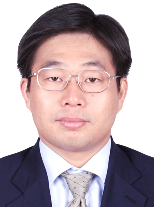
\includegraphics[width=1in,height=1.25in,clip,keepaspectratio]{fig/authors/CASun.pdf}}]{Chang-ai Sun} is a Professor in the School of Computer and Communication Engineering, University of Science and Technology Beijing.
Before that, he was an Assistant Professor at Beijing Jiaotong University, China, a postdoctoral fellow at the Swinburne University of Technology, Australia, and a postdoctoral fellow at the University of Groningen, The Netherlands. He received the bachelor degree in Computer Science from the University of Science and Technology Beijing, China, and the PhD degree in Computer Science from Beihang University, China.
His research interests include software testing, program analysis, and Service-Oriented Computing.
\end{IEEEbiography}
\vspace{-10ex}
\begin{IEEEbiography}[{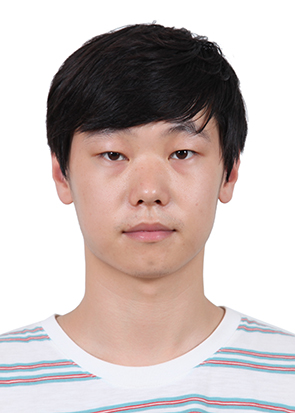
\includegraphics[width=1in,height=1.25in,clip,keepaspectratio]{fig/authors/HPDai.jpg}}]{Hepeng Dai} is a PhD student in the School of Computer and Communication Engineering, University of Science and Technology Beijing, China. He received the master degree in Software Engineering from University of Science and Technology Beijing, China and the bachelor degree in Information and Computing Sciences from China University of Mining and Technology, China. His current research interests include software testing and debugging.
\end{IEEEbiography}
\vspace{-10ex}
\begin{IEEEbiography}[{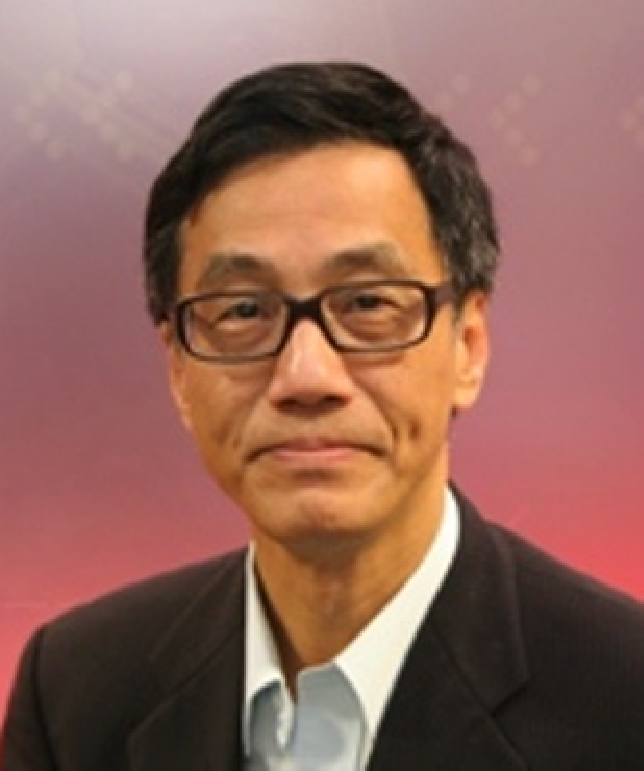
\includegraphics[width=1in,height=1.25in,clip,keepaspectratio]{fig/authors/TYChen.pdf}}]{Tsong Yueh Chen} is a Professor of Software Engineering at the Department of Computer Science and Software Engineering in Swinburne University of Technology. He received his PhD in Computer Science from The University of Melbourne, the MSc and DIC from Imperial College of Science and Technology, and BSc and MPhil from The University of Hong Kong. He is the inventor of metamorphic testing and adaptive random testing.
\end{IEEEbiography}
\vspace{-10ex}
\begin{IEEEbiography}[{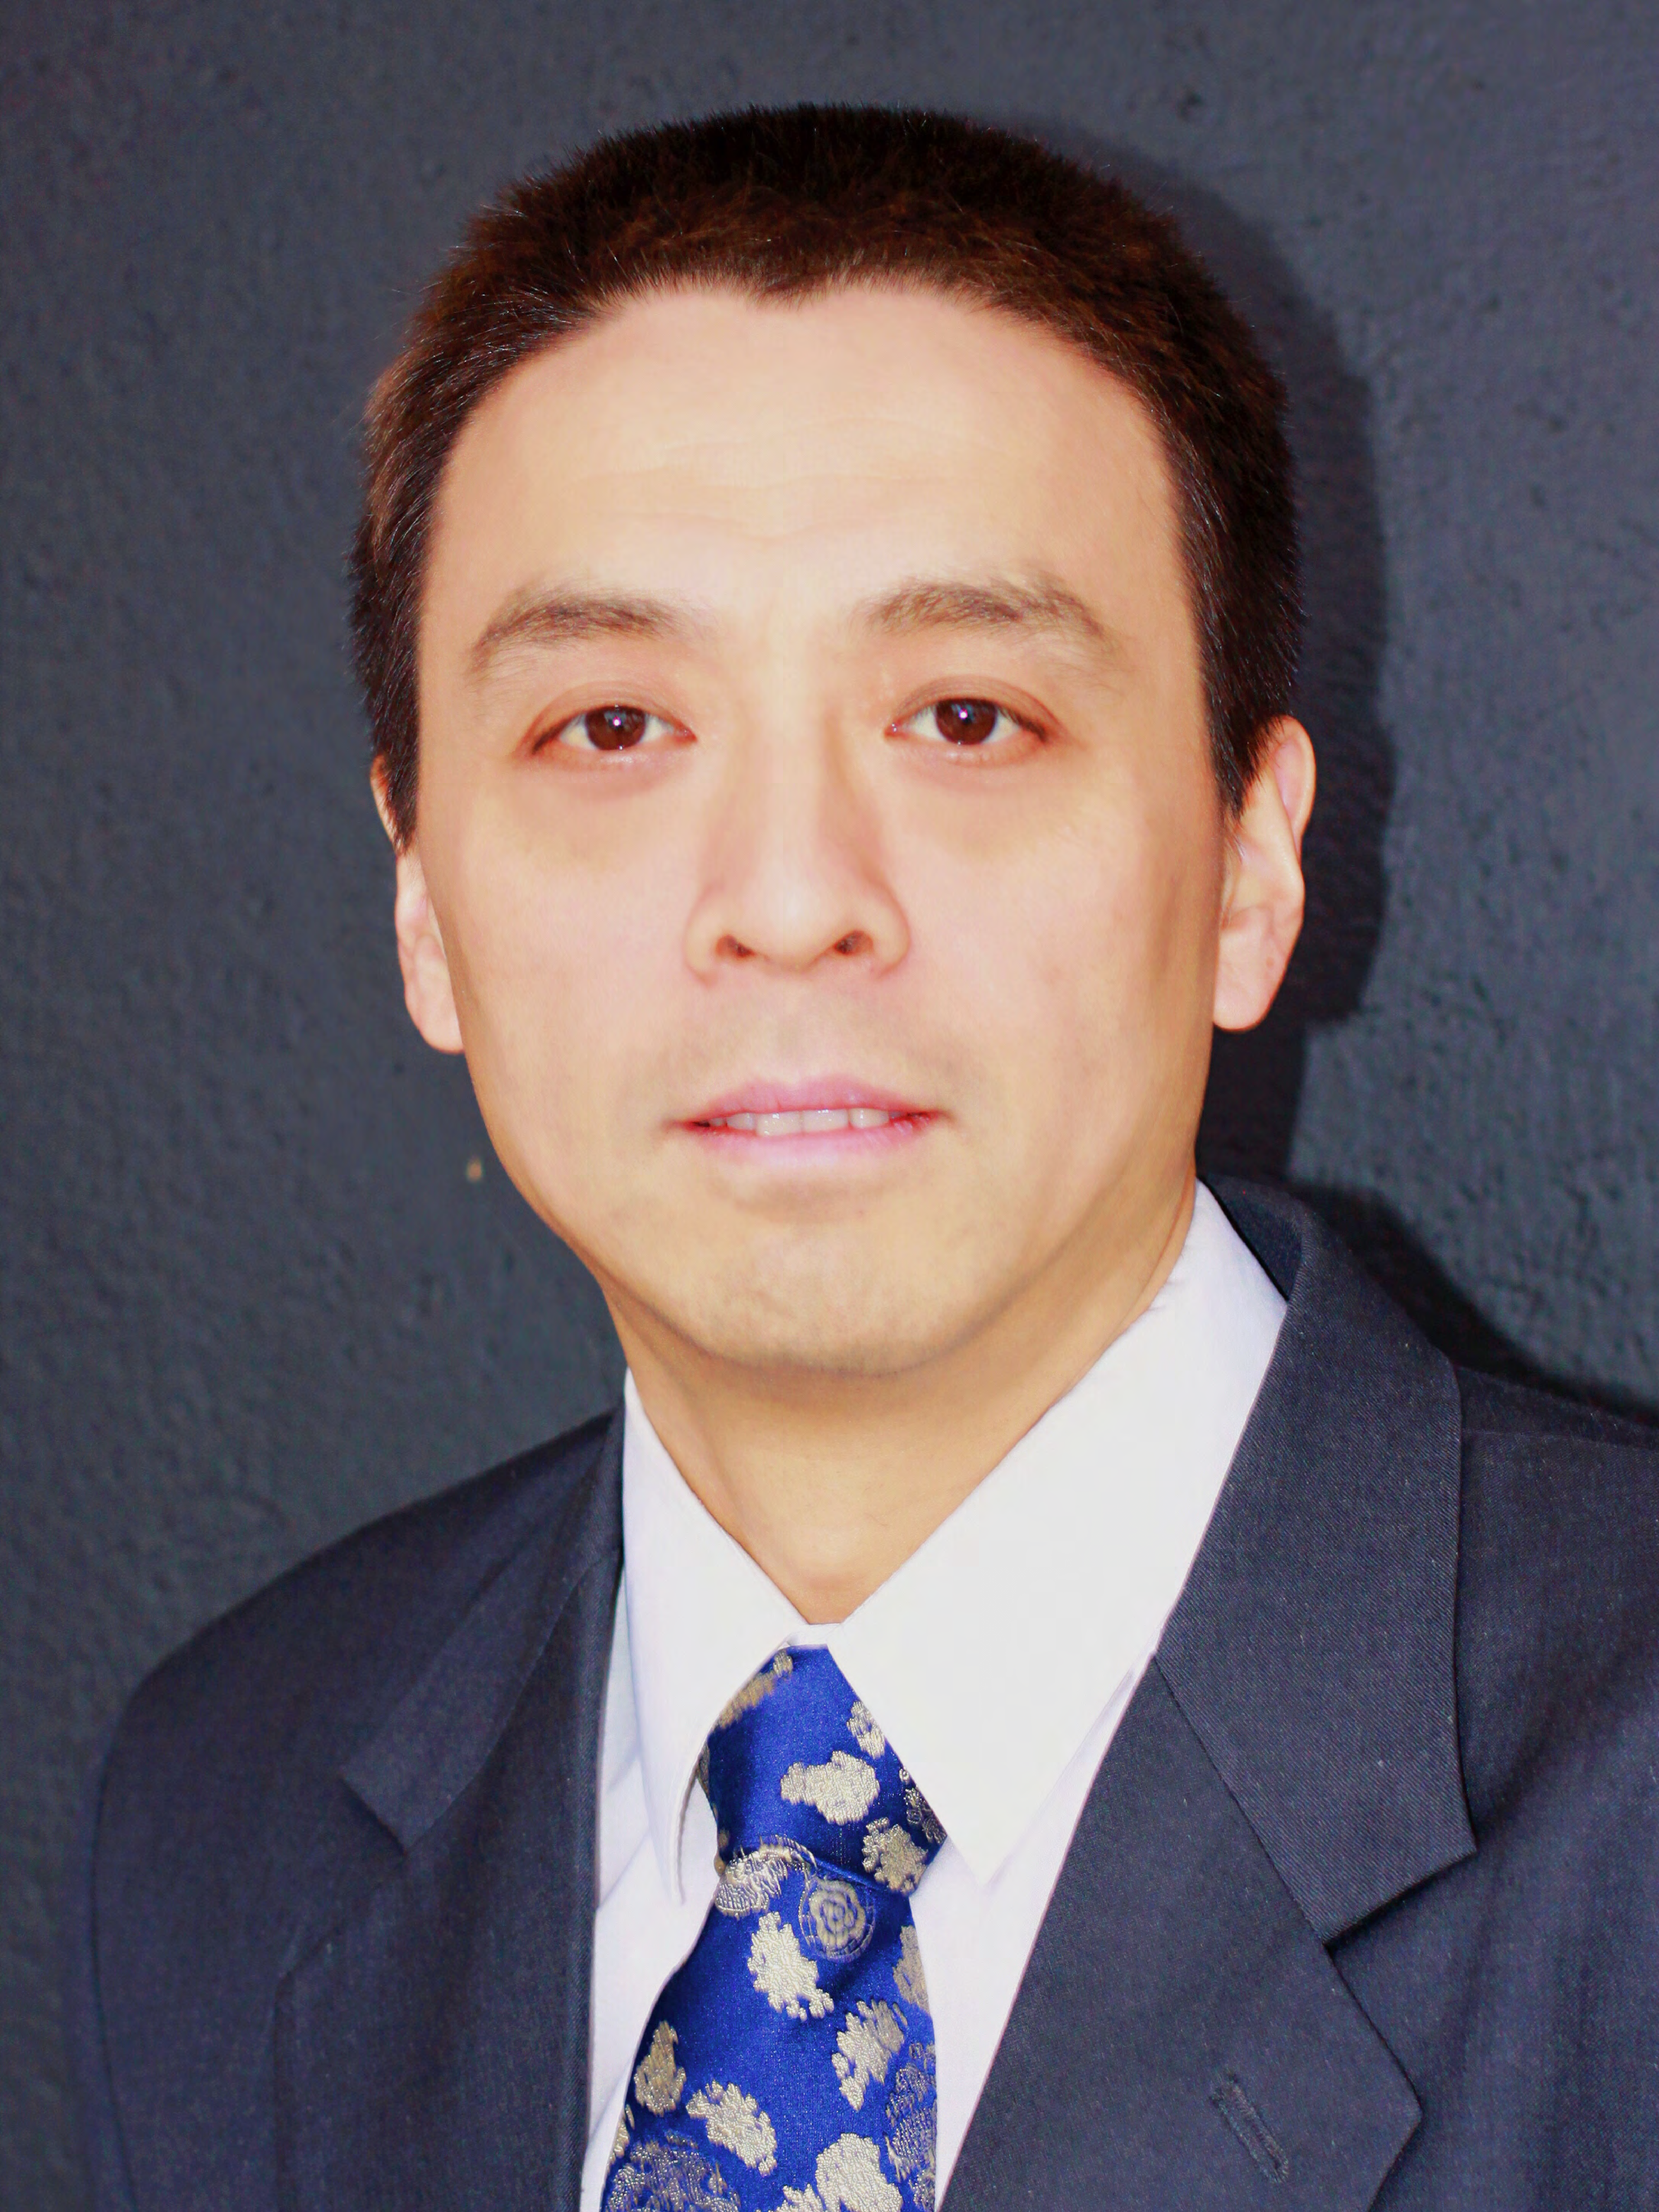
\includegraphics[width=1in,height=1.25in,clip,keepaspectratio]{fig/authors/HLiu.pdf}}]{Huai Liu} is a Lecturer of Information Technology at the College of Engineering \& Science in Victoria University, Melbourne, Australia. Prior to joining VU, he worked as a research fellow at RMIT University and a research associate at Swinburne University of Technology. He received the BEng in physioelectronic technology and MEng in communications and information systems, both from Nankai University, China, and the PhD degree in software engineering from the Swinburne University of Technology, Australia. His current research interests include software testing, cloud computing, and end-user software engineering.
\end{IEEEbiography}

\end{document}
